\ifdefined \wholebook \else\documentclass[oneside]{book}\usepackage{EdlBook}\graphicspath{{figures/}}
\addto\captionsicelandic{\renewcommand{\chaptername}{Kafli}}
%\setsecnumdepth{chapter}
\begin{document}
%%%
%
\setcounter{chapter}{11} % one less than this chapter
%
%%%
\fi
%%%%%%%%%%%%%%%%%%%%%%%%%%%%%%%%
%      CHAPTER TEXT GOES BELOW
%%%%%%%%%%%%%%%%%%%%%%%%%%%%%%%%

\renewcommand{\thefigure}{\arabic{figure}}
\counterwithout{equation}{chapter}

\chapter{Bylgjur}

\section{Hvað er bylgja?}

\begin{tcolorbox}
\begin{definition}
Látum $\psi(x,t)$ lýsa fráviki hlutar frá jafnvægisstöðu sinni sem fall af staðsetningu, $x$ og tíma, $t$. Við segjum að hluturinn sé á \textbf{bylgjuhreyfingu} með \textbf{bylgjuhraða} $c$ ef frávikið uppfyllir \textbf{bylgjujöfnuna}:
\begin{align*}
    \frac{\partial^2\psi}{\partial t^2} = c^2 \frac{\partial^2 \psi}{\partial x^2}.
\end{align*}
\end{definition}
\end{tcolorbox}

Ef við notum punktrithátt fyrir $\frac{\partial}{\partial t}$ og merktrithátt fyrir $\frac{\partial}{\partial x}$ þá getum við skrifað bylgjujöfnuna sem:
\begin{align*}
    \Ddot{\psi} = c^2 \psi''
\end{align*}
Við athugum að einingarnar á $\psi$ eru $\left[ \psi \right] = \si{m}$ því það lýsir fjarlægð frá jafnvægisstöðu. Bylgjuhraðinn $c$ er almennt háður efninu eða \textbf{miðlinum} sem bylgjan berst í. Við þurfum síðan að taka fram tvær mismunandi gerðir af hreyfingarstefnum sem að bylgjur geta haft:

\begin{tcolorbox}
\begin{definition}
Við segjum að bylgja sé
\begin{enumerate}[label = \textbf{(\roman*)}]
    \item \textbf{langsbylgja} ef hreyfing agnanna í miðlinum er þvert á hreyfistefnu bylgjunnar.
    \item \textbf{þverbylgja} ef hreyfing agnanna í miðlinum er samsíða hreyfistefnu bylgjunnar.
\end{enumerate}
\end{definition}
\end{tcolorbox}

Til dæmis eru sveiflur í gítarstreng dæmi um þverbylgjur. Annað dæmi um þverbylgjur eru gárurnar sem myndast í yfirborði vatns eftir að stein er sleppt ofan í vatnið. Hljóð er síðan dæmi um langsbylgjur.

\begin{figure}[H]
    \centering
    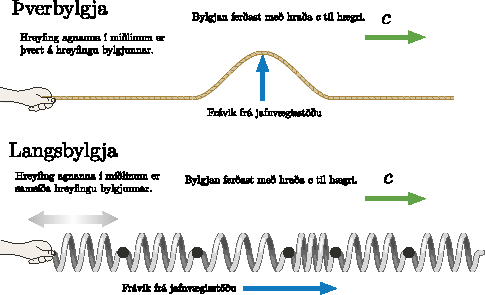
\includegraphics{figures/langs-thver.pdf}
\end{figure}

\section{Staðbylgjur á streng} 

\begin{comment}
Við skulum byrja á því að skoða staðbylgjur á streng. Við byrjum á einfaldasta fyrirbærinu. Við byrjum á því að skoða gítarstreng sem er festur í báða endana og síðan sleginn. Þá byrjar hann að sveiflast fram og til baka. 
\end{comment}

\begin{tcolorbox}
\begin{theorem}
Lítum á streng með massa $m$ af lengd $\ell$ sem festur er í báða enda. Látum $\mu = \frac{m}{\ell}$ vera línulegan þéttleika strengsins og látum togkraftinn í vírnum vera $T$. Látum $y = y(x,t)$ tákna lóðrétt frávik strengsins frá jafnvægisstöðu sinni bæði sem fall af tíma, $t$, og láréttri staðsetningu, $x \in [0,\ell]$. Þá uppfyllir frávikið á strengnum eftirfarandi bylgjujöfnu með bylgjuhraða $c = \sqrt{\frac{T}{\mu}}$
\begin{align*}
    \Ddot{y} = \frac{T}{\mu} y''
\end{align*}
\end{theorem}
\end{tcolorbox}


\textbf{Útleiðsla:} Skoðum lítinn bút af strengnum milli $x$ og $x + \Delta x$ við einhvern ótiltekinn tíma $t$.

\begin{figure}[H]
    \centering
    \vspace{-0.4cm}
    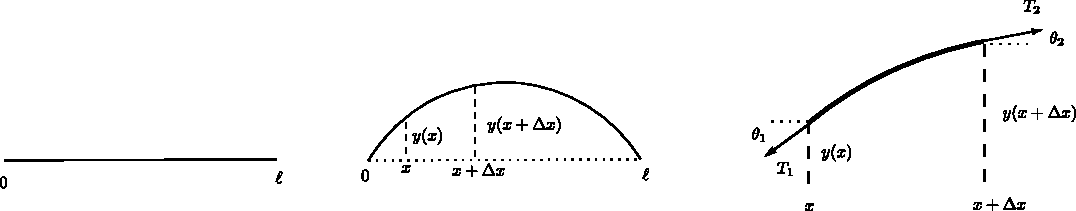
\includegraphics[scale = 0.9]{figures/strengur-deriv.pdf}
    \label{fig:standing-waves}
\end{figure}

\vspace{-0.4cm}
Þá er massinn í þessum litla bút af strengnum gefinn með $\frac{\Delta x}{\ell} m = \mu \Delta x$. Kraftajafnan verður þá:
\begin{align*}
   \mu \Delta x \begin{pmatrix}  \Ddot{x} \\  \Ddot{y} \end{pmatrix} = \begin{pmatrix} T_2 \cos\theta_2 - T_1 \cos\theta_1 \\ T_2 \sin\theta_2 - T_1\sin\theta_1 \end{pmatrix}
\end{align*}

Strengurinn er ekki að færast til í láréttu stefnuna svo að $\Ddot{x} = 0$. Ef við notum síðan nálgunina að $\cos\theta \approx 1$ þá sjáum við að efri jafnan gefur okkur að $T_2 = T_1$ svo að togkrafturinn í vírnum er um það bil fastur meðfram strengnum og þar með er $T = T_1 = T_2$. Neðri jafnan er frekar athyglisverð því þar er $\Ddot{y} \neq 0$ þar sem að strengurinn lyftist upp og hefur því færst úr stað. Við notum þá nálgunina $\tan\theta = \frac{\sin\theta}{\cos\theta} \approx \frac{\theta}{1} = \theta \approx \sin\theta$. En $\tan\theta = \frac{dy}{dx} = y'$ samkvæmt skilgreiningu á hallatölu svo að við ályktum að:
\begin{align*}
    \mu \Delta x \Ddot{y} = T\left( y'(x+\Delta x,t) - y'(x,t) \right)
\end{align*}
En þar með ályktum við að:
\begin{align*}
    \Ddot{y} = \frac{T}{\mu} \frac{y'(x+\Delta x,t)-y'(x,t)}{\Delta x} = \frac{T}{\mu} y''
\end{align*}
Við höfum þar með sýnt að staðbylgjur á streng uppfylla bylgjujöfnuna:
\begin{align*}
    \Ddot{y} = \frac{T}{\mu} y''
\end{align*}

\qed

Það er líka hægt að leiða út bylgjuhraðann með víddargreiningu. Þá er $c = m^\alpha \ell^\beta T^\gamma$ og við fáum að:
\begin{align*}
  \si{m^1}\si{s^{-1}} = \frac{\si{m}}{\si{s}} = [c] = [m]^\alpha [\ell]^\beta [T]^\gamma = \left( \si{kg} \right)^\alpha \left( \si{m} \right)^\beta \left( \frac{\si{kg.m}}{\si{s^2}} \right)^\gamma = (\si{kg})^{\alpha + \gamma} (\si{m})^{\beta + \gamma} (s)^{-2\gamma}
\end{align*}
sem gefur okkur því jöfnuhneppið:
\begin{align*}
    \begin{cases}
    1 = \beta + \gamma \\
    0 = \alpha + \gamma \\
    -1 = -2\gamma
    \end{cases}
\end{align*}
En þar með getum við ályktað að $\gamma = \frac{1}{2}$, $\beta = \frac{1}{2}$ og $\alpha = -\frac{1}{2}$ en það gefur okkur því að $c = \sqrt{\frac{T\ell}{m}} = \sqrt{\frac{T}{\mu}}$.

\begin{comment}
Við athugum síðan að þar sem að $\Delta x$ er valið mjög lítið þá er $\theta_2 \approx \theta_1 + \Delta \theta$ þar sem $\Delta \theta$ er lítil stærð. En þá gefur summuregla hornafalla að:
\begin{align*}
    \cos(\theta_2) \approx \cos(\theta_1 + \Delta \theta) = \cos(\theta_1)\cos(\Delta \theta) - \sin(\theta_1)\sin(\Delta \theta) \approx \cos(\theta_1) - \sin(\theta_1) \Delta \theta
\end{align*}
En þar með sjáum við að kraftajafnan í lárettu stefnuna gefur:
\begin{align*}
    0 = T_2 \cos(\theta_2) - T_1 \cos(\theta_1) \approx T_2 \cos(\theta_1) - T_2 \sin(\theta_1)\Delta \theta - T_1 \cos(\theta_1)
\end{align*}
En þessi jafna verður að gilda fyrir öll $\Delta \theta$ sama hversu lítil og við veljum þau svo við ályktum að til þess að lárétta kraftajafnan gangi upp þá þarf:
\begin{align*}
    T_2 \sin(\theta_1) \explain{\Delta \theta}{\approx 0} = (T_1 - T_2) \cos(\theta_1) \implies T_1 \approx T_2
\end{align*}
Svo togkrafturinn er svo gott sem sá sami, $T$, alls staðar í strengnum. En þá 
\end{comment}


\section{Hljóðbylgjur}

\begin{tcolorbox}
\begin{theorem}
Lítum á ræmu af kjörgasi með rúmmál $V_0$ sem er við þrýsting $P_0$ og hefur hitastig $T_0$. Látum eðlismassa gasins vera $\rho_0$ og látum $z = z(x,t)$ tákna frávik kjörgasins frá upphafsstaðsetningunni. Þá uppfyllir frávikið bylgjujöfnuna, $\Ddot{z} = \frac{P_0}{\rho_0} z''$, með bylgjuhraða $c = \sqrt{\frac{P_0}{\rho_0}}$
\end{theorem}
\end{tcolorbox}

\begin{comment}
\begin{figure}[H]
    \centering
    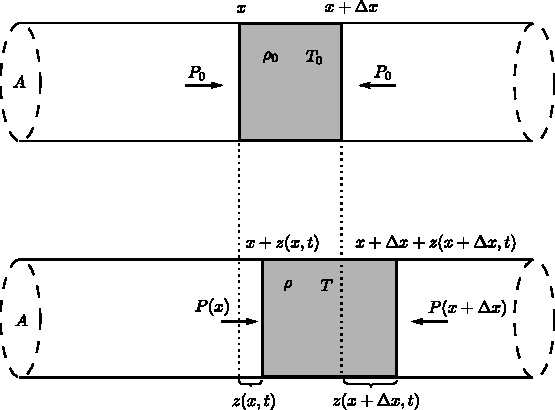
\includegraphics[scale = 0.8]{figures/loft-pipa.pdf}
    \label{fig:loft-belgur}
\end{figure}
\end{comment}

\begin{minipage}{\linewidth}

\begin{wrapfigure}{r}{3in}
\vspace{-0.5cm}
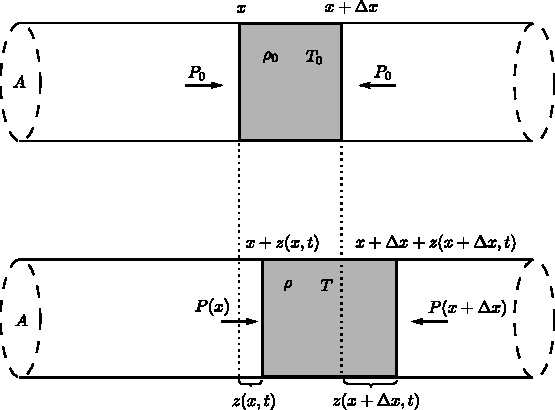
\includegraphics[width=2.7in]{figures/loft-pipa.pdf}
\end{wrapfigure}

\textbf{Útleiðsla:} Skoðum ræmu af lofti með þverskurðarflatarmál $A$ og af lengd $\Delta x$ sem er í upphafi kyrr (áður en að hljóðbylgjan berst á þennan stað). Þá er þrýstingurinn á báðar hliðar ræmunnar jafn $P_0$ og loftið í ræmunni hefur eðlismassa $\rho_0$ og hitastig $T_0$. Við höfum þá að massinn í þessari litlu loftræmu er $m = \rho_0 A \Delta x$. Eftir að hljóðbylgjan berst á þennan stað þá mun loftið færast frá jafnvægisstöðunni sinni um einhverja vegalengd þannig að vinstri endinn færist frá $x$ yfir í $x + z(x,t)$ og hægri endinn færist frá $x + \Delta x$ yfir í $x + \Delta x + z(x+\Delta x, t)$. En þar með mun rúmmál ræmunnar breytast frá því í upphafi að vera $V_0$ yfir í að vera:
\end{minipage}

\begin{align*}
    V &= A\Bigg( \Delta x + z(x+\Delta x,t) - z(x,t) \Bigg) = A \Delta x \Bigg( 1 + \frac{z(x+\Delta x,t)-z(x,t)}{\Delta x} \Bigg) = V_0 \left(1 + z'\right).
\end{align*}
Þar sem að við höfum notað skilgreininguna á afleiðunni.
\begin{comment}
En þar sem að rúmmálið hefur breyst þá hefur eðlismassinn einnig breyst (heildarmassinn í ræmunni er samt sá sami). Við höfum þá að:
\begin{align*}
    \rho = \frac{m}{V} = \frac{m}{V_0(1+z')} = \rho_0\left( 1 + z' \right)^{-1} \approx \rho_0\left( 1 - z'\right)
\end{align*}
Þar sem að við höfum notað nálgunina $(1+x)^n \approx 1 + nx$ ef $x \ll 1$ er lítið.
\end{comment}
En þar sem að rúmmálið hefur breyst þá hefur þrýstingurinn líka breyst! Við getum notað gaslögmálið $PV = nRT$ (sem við munum leiða út síðar í kafla 15 um Varmafræði) til þess að athuga hvernig þrýstingurinn breytist þegar rúmmálið breytist. Á þessum tímapunkti ætlum við að gera sömu mistök og Isaac Newton (ekki leiðum að líkjast!) í útleiðslunni og segja að hitastigsbreytingin sé mjög lítil svo $T \approx T_0$ (það er ekki alveg satt!) og að þess vegna sé $PV = nRT = P_0 V_0$ svo að við fáum að:
\begin{align*}
    P = \frac{P_0 V_0}{V} = \frac{P_0 V_0}{V_0 ( 1+ z')} = P_0 \left( 1 + z' \right)^{-1} \approx P_0(1 - z')
\end{align*}
Þar sem við höfum notað nálgunina $(1+x)^n \approx 1 + nx$ fyrir $x \ll 1$ sem er lítið. En þá gefur kraftajafnan að:
\begin{align*}
    \rho_0 V_0 \Ddot{z} = m \Ddot{z} =  \Bigg(P(x)-P(x+\Delta x)\Bigg)A = P_0\Bigg( z'(x+\Delta x,t) - z'(x,t) \Bigg)A = P_0\Bigg( \frac{z'(x+\Delta x, t)-z'(x,t)}{\Delta x} \Bigg) V_0
\end{align*}
Við notum síðan skilgreininguna á afleiðunni ásamt því að stytta út $V_0$ til þess að álykta að $\Ddot{z} = \frac{P_0}{\rho_0} z''$.
\qed 

\vspace{0.5cm}

Við sjáum þá að með þessari aðferð (sem er upphaflega eftir Newton) fáum við að hraði hljóðsins er:
\begin{align*}
    v_{\text{hljóð}} = \sqrt{\frac{P_0}{\rho_{\text{loft}}}} = \sqrt{\frac{\SI{101.3}{kPa}}{\SI{1.225}{kg/m^3}}} = \SI{288}{m/s}.
\end{align*}
Sem er í nærri lagi við að viðtekið gildi á hraða hljóðsins í lofti $v_{\text{hljóð}} = \SI{343}{m/s}$. Reyndar er auðvelt að laga mistökin sem Newton gerði (eftir að við lærum hvað óvermið ferli er í kafla 15 um Varmafræði). Það kemur í ljós að hitastigið á loftinu er að breytast nógu mikið til þess að nálgunin $T \approx T_0$ sé ekki nógu góð! Reyndar kemur í ljós að það er til önnur varðveitt stærð sem nefnist óvermnióbreytan, $PV^\gamma$, þar sem $\gamma$ er fasti sem er háður sameindauppbyggingu kjörgasins og nefnist Laplacefastinn eða óvermnisstuðullinn. Fyrir loft er hægt að sýna að $\gamma_{\text{loft}} = \frac{7}{5}$. Með því að laga útleiðsluna þá getum við sýnt að þá verður hljóðhraðinn gefinn með:
\begin{align*}
    c = \sqrt{\frac{\gamma P_0}{\rho_0}}
\end{align*}
En þá fæst að $v_{\text{hljóð}} = \sqrt{\frac{\gamma_{\text{loft}}P_0}{\rho_{\text{loft}}}} = \SI{340}{m/s}$.

\newpage

\section{Að leysa bylgjujöfnuna}

Í kaflanum um einfalda sveifluhreyfingu þá sýndum við að lausnir á diffurjöfnunni $\Ddot{z} = -\omega^2 z$ voru gefnar með $z(t) = A\sin(\omega t + \varphi)$ og við skilgreindum útslag sveiflunnar, $A$, sveiflutímann, $T$, og sveiflutíðnina, $\omega$. Það kemur í ljós að bylgjujafnan er í rauninni bara það sem við fáum þegar við setjum saman sveifluhreyfingu í tíma og rúmi, þ.e.a.s.~lausnir bylgjujöfnunnar, $\psi(x,t)$, munu sveiflast með einfaldri sveifluhreyfingu sem fall af tíma og sem fall af stöðu!

\begin{tcolorbox}
\begin{theorem}
Grunnlausnir bylgjujöfnunnar $\Ddot{\psi} = c^2 \psi''$ eru gefnar með:
\begin{align*}
    \psi(x,t) = A\sin(kx - \omega t + \varphi_0)
\end{align*}
Þar sem $\omega$ er sveiflutíðni; $A$ er útslag; $\varphi_0$ er fasahorn og $k := \frac{\omega}{c}$ er \textbf{bylgjutala} bylgjunnar.
\end{theorem}
\end{tcolorbox}

\textbf{Útleiðsla:} Við diffrum bara. Athugum að:
\begin{align*}
    \dot{\psi} = -\omega A \cos(kx - \omega t + \varphi_0), \hspace{0.8cm} \text{þannig að} \hspace{0.8cm} \Ddot{\psi} = -\omega^2 A \sin(kx - \omega t + \varphi_0).
\end{align*}
Athugum síðan að:
\begin{align*}
    \psi' = -Ak \cos(kx - \omega t + \varphi_0), \hspace{0.8cm} \text{þannig að} \hspace{0.8cm} \psi'' = -Ak^2 \sin(kx - \omega t + \varphi_0).
\end{align*}
En þar með höfum við að:
\begin{align*}
    \Ddot{\psi} = -\omega^2 A\sin(kx-\omega t + \varphi_0) = -c^2k^2 \sin(kx - \omega t + \varphi_0) = c^2 \psi''.
\end{align*}
Þar sem við höfum notað skilgreininguna á bylgjutölunni, $\omega = kc$.

\qed

\begin{tcolorbox}
\begin{definition}
Látum $\psi(x,t) = A\sin(kx - \omega t + \varphi_0)$ vera grunnlausn á bylgjujöfnunni.
\begin{figure}[H]
    \centering
    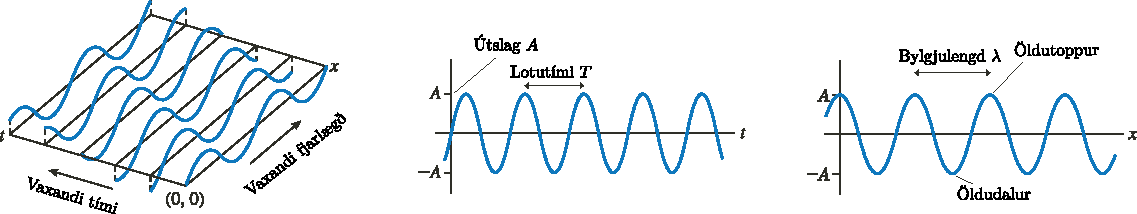
\includegraphics[scale = 0.8]{figures/waves.pdf}
\end{figure}
\begin{enumerate}[label = \textbf{(\roman*)}]
    \item Við segjum að \textbf{lotutími} bylgjunnar sé $T = \frac{2\pi}{\omega}$.
    \item Við segjum að \textbf{bylgjulengd} bylgjunnar sé $\lambda = \frac{2\pi}{k}$.
    \item Við segjum að \textbf{tíðni} bylgjunnar sé $f = \frac{1}{T} = \frac{\omega}{2\pi}$.
\end{enumerate}
\end{definition}
\end{tcolorbox}

Reyndar ættum við líka að minnast á að við hugsum um lotutímann sem tímann sem líður á milli hverar sveiflu sem fall af tíma og bylgjulengdin er vegalengdin sem líður milli hverar sveiflu (það er að segja hversu langt er á milli öldutoppanna).

\begin{tcolorbox}
\begin{theorem}
Látum $c$ vera bylgjuhraða bylgju með bylgjulengd $\lambda$ og tíðni $f$. Þá gildir að:
\begin{align*}
    c = \lambda f.
\end{align*}
\end{theorem}
\end{tcolorbox}

\textbf{Útleiðsla:} Við fáum að:
\begin{align*}
    c = \frac{\omega}{k} = \frac{2\pi f}{\frac{2\pi}{\lambda}} = \lambda f.
\end{align*}
\qed

\section{Afl og styrkur}

\begin{tcolorbox}
\begin{definition}
Látum $\Delta E$ tákna breytingu á orku á kerfi vegna vinnunnar sem er unnin á því á tímanum $\Delta t$. Þá er \textbf{aflið}, $P$, skilgreint þannig að:
\begin{align*}
    P = \frac{\Delta E}{\Delta t}.
\end{align*}
\end{definition}
\end{tcolorbox}

Þetta er í rauninni meðalaflið á tímanum $\Delta t$. Við getum líka skrifað aflið á formi örsmæða. Þá er yfirleitt skipt orkubreytingunni út fyrir vinnunna þannig að: $P = \frac{d W}{dt}$. Við sjáum að $[P] = \si{J/s} = \si{W}$ en sú stærð hefur fengið nafnið Watt til heiðurs skoska verkfræðingnum James Watt. Það er hinsvegar eðlilegt að tala um afl tiltekins krafts svo við athugum að:

\begin{tcolorbox}
\begin{theorem}
Látum $\vec{F}$ tákna fastann kraft sem verkar á hlut með hraðavigur $\vec{v}$. Afl kraftsins er þá
\begin{align*}
    P = \Vec{F} \cdot \Vec{v}
\end{align*}
\end{theorem}
\end{tcolorbox}

\textbf{Útleiðsla:} Við fáum að:
\begin{align*}
    P = \frac{dW}{dt} = \frac{d}{dt}\left( \Vec{F} \cdot \Delta \Vec{s} \right) = \explain{\frac{d\Vec{F}}{dt}}{=0} \cdot \Delta \Vec{s} + \Vec{F} \cdot \explain{\frac{d\Delta \Vec{s}}{dt}}{= \vec{v}} = \Vec{F} \cdot \Vec{v}.
\end{align*}
Þar sem við höfum notað að $\frac{d \Vec{F}}{dt} = 0$ því $\Vec{F}$ er fastur kraftur.
\qed


\begin{tcolorbox}
\begin{definition}
Látum $P$ vera afl bylgju og látum $A$ vera yfirborðsflatarmál sem bylgjan breiðist út í gegnum. \textbf{Bylgjustyrkur} bylgjunnar er táknaður með $I$ og skilgreindur þannig að:
\begin{align*}
    I = \frac{P}{A}
\end{align*}
\end{definition}
\end{tcolorbox}

Ef við erum með uppsprettu sem er kúlusamhverf, og sendir því bylgjur í allar áttir, þá mun aflið dreifast jafnt yfir kúlu með yfirborðsflatarmál $A = 4\pi r^2$ í fjarlægð $r$ frá uppsprettunni. Þá höfum við að bylgjustyrkurinn er gefinn með $I = \frac{P}{4\pi r^2}$ í fjarlægð $r$ frá uppsprettunni. \\

Við komum nú loksins að ljótustu jöfnu sem þið munið nokkru sinni læra á skólagögnu ykkar í MR, þ.e.a.s.~skynstyrksjöfnunni:

\begin{tcolorbox}
\begin{definition}
Gerum ráð fyrir að við höfum hljóðuppsprettu með hljóðstyrk $I$. Þá er \textbf{skynstyrkur hávaðans}
\begin{align*}
    \beta = \beta_0 \log_{10}\left(\frac{I}{I_0}\right)
\end{align*}
Þar sem $\beta_0 = \SI{10}{dB}$ og $I_0 = \SI{e-12}{W/m^2}$.
\end{definition}
\end{tcolorbox}


Sálfræðirannsóknir í hljóðeðlisfræði hafa leitt í ljós að fólk segir að hljóð sé tvöfalt hærra við það að skynstyrkur hávaðans hækki um $\SI{10}{dB}$. Hinsvegar þá eykst skynstyrkur hávaðans aðeins um $\SI{3}{dB}$ við það að tvöfalda afl uppsprettunnar, $P_2 = 2P_1$, eins og við skulum nú sýna:
\begin{align*}
    \beta_2 - \beta_1 = \beta_0 \log_{10}\left( \frac{P_2}{A I_0} \right) - \beta_0 \log_{10}\left( \frac{P_1}{A I_0} \right) = \beta_0 \log_{10}\left( \frac{P_2}{P_1} \right) = \beta_0 \log_{10}(2) = \SI{3}{dB}.
\end{align*}

\section{Dopplerhrif}

\subsection*{Kyrrstæður viðtakandi og uppspretta sem hreyfist}

\begin{tcolorbox}
\begin{theorem}
Látum $f_0$ vera tíðnina á bylgjunum sem að uppspretta sendir frá sér. Látum uppsprettuna fjarlægjast kyrrstæðan viðtakanda (1) og nálgast kyrrstæðan viðtakanda (2) með hraða $u$. Þá gildir að tíðnin sem viðtakendurnir heyra er gefin með:
\begin{align*}
    f_1 = \left( \frac{c}{c + u} \right)f_0, \hspace{1cm} f_2 = \left( \frac{c}{c - u} \right)f_0
\end{align*}
\begin{figure}[H]
    \centering
    \vspace{-0.5cm}
    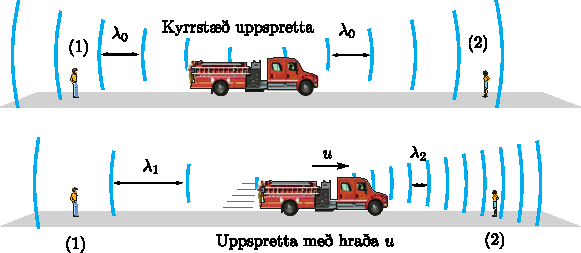
\includegraphics[scale = 0.8]{figures/doppler-brunabill.pdf}
\end{figure}
\end{theorem}
\end{tcolorbox}

\textbf{Útleiðsla:} Látum $T_0 = \frac{1}{f_0}$ tákna tímann sem líður milli þess að uppsprettan sendir frá sér bylgju. Þá mun bylgjulengdin lengjast (fyrir viðtakanda 1) samkvæmt:
\begin{align*}
    \lambda_1 = \lambda_0 + uT_0
\end{align*}
Þar sem að uppsprettan mun hafa færst til um vegalengd $uT_0$ milli þess að senda frá sér bylgjurnar. En hraði hljóðsins, $c$, er óbreyttur í miðlinum svo við ályktum að:
\begin{align*}
    f_1 = \frac{c}{\lambda_1} = \frac{c}{\lambda_0 + u T_0} = \frac{c}{\lambda_0 + \frac{u}{f_0}} = \frac{cf_0}{\lambda_0 f_0 + u} = \left(\frac{c}{c+u} \right)f_0.
\end{align*}
Með sömu reikningum fæst að $f_2 = \left(\frac{c}{c-u}\right) f_0$. \qed


\subsection*{Viðtakandi sem hreyfist og kyrrstæð uppspretta}

\begin{tcolorbox}
\begin{theorem}
Látum $f_0$ vera tíðnina á bylgjunum sem að kyrrstæð uppspretta sendir frá sér. Látum viðtakanda (1) nálgast uppsprettuna og látum viðtakanda (2) fjarlægjast uppsprettuna með hraða $v$. Þá gildir að tíðnin sem viðtakendurnir heyra er gefin með:
\begin{align*}
    f_1 = \left( \frac{c-v}{c} \right)f_0, \hspace{1cm} f_2 = \left( \frac{c+v}{c} \right)f_0
\end{align*}
\begin{figure}[H]
    \centering
    \vspace{-0.5cm}
    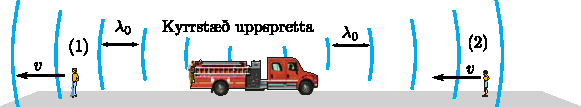
\includegraphics[scale = 0.8]{figures/doppler-brunabill-kyrr.pdf}
\end{figure}
\end{theorem}
\end{tcolorbox}

\textbf{Útleiðsla:} Látum $T_0 = \frac{1}{f_0}$ tákna tímann sem líður milli þess að uppsprettan sendir frá sér bylgju og látum $T_1$ tákna tímann sem líður milli þess að viðtakandi (1) greinir bylgjurnar. Þá er vegalengdin sem viðtakandinn ferðast á milli þess að greina bylgjuna $\lambda_0 + vT_1$ en vegalengdin sem bylgjan þarf að ferðast á sama tíma er þá $cT_1$. Við fáum því að:
\begin{align*}
    \lambda_0 + vT_1 = cT_1 \implies T_1 (c-v) = \lambda_0 \implies T_1 = \frac{\lambda_0}{c-v} \implies f_1 = \frac{1}{T_1} = \frac{c-v}{\lambda_0} = \left(\frac{c-v}{c}\right) f_0.
\end{align*}
Sömu reikningar gefa síðan að $f_2 = \left(\frac{c+v}{c} \right)f_0$.
\qed

\subsection*{Allsherjarjafnan}

Ef við setjum þessar tvær hugmyndir saman þá fáum við:

\begin{tcolorbox}
\begin{theorem}
Látum $f_0$ vera tíðnina sem að uppspretta með hraða $u$ sendir frá sér í áttina að viðtakanda með hraða $v$. Þá gildir að tíðnin sem viðtakandinn heyrir er gefin með:
\begin{align*}
    f = \left( \frac{c \pm v}{c \pm u} \right)f_0
\end{align*}
Þar sem $c$ táknar bylgjuhraðann í miðlinum, $v$ táknar hraða viðtakandans og $u$ táknar hraða uppsprettunnar. Formerkið á $v$ er jákvætt ef viðtakandinn er að ferðast í áttina að uppsprettunni en neikvætt ef viðtakandinn er að ferðast frá uppsprettunni. Formerkið á $u$ er jákvætt ef uppsprettan er að ferðast í burtu frá viðtakandanum en neikvætt ef uppsprettan er að ferðast að viðtakandanum.
\end{theorem}
\end{tcolorbox}

\textbf{Útleiðsla:} Þetta fæst einfaldlega með því að margfalda saman niðurstöðurnar í lögmálunum tveim á undan:
\begin{align*}
    f = \left( \frac{c\pm v}{c} \right)\left( \frac{c}{c\pm u} \right)f_0 = \left( \frac{c \pm v}{c \pm u} \right)f_0.
\end{align*}
\qed

Við tökum síðan saman í litla töflu þessi fjögur tilvik og hvernig þau líta út:

\begin{table}[h!]
  \centering
  \begin{tabular}{ | c | m{5.2cm} | m{2.5cm} | }
    \hline
    \textbf{Mynd} & \hspace{1.9cm} \textbf{Lýsing} & \hspace{0.4cm} \textbf{Tíðni} \\ \hline
    \begin{minipage}{.4\textwidth}
    \vspace{0.3cm}
    \centering
      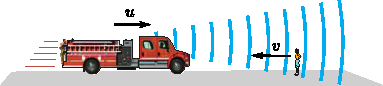
\includegraphics[width=0.95\linewidth]{figures/doppler-tilvik1.pdf}
    \vspace{0.3cm}
    \end{minipage}
    &
      Viðtakandi nálgast uppsprettu. \par Uppspretta nálgast viðtakanda.
    & 
      \begin{align*}
          f = \left( \frac{c + v}{c - u} \right)f_0
      \end{align*}
    \\ \hline
    \begin{minipage}{.4\textwidth}
    \vspace{0.3cm}
    \centering
      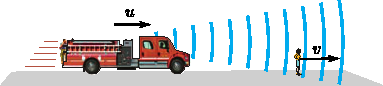
\includegraphics[width=0.95\linewidth]{figures/doppler-tilvik12.pdf}
    \vspace{0.3cm}
    \end{minipage}
    &
          Viðtakandi fjarlægist uppsprettu. \par Uppspretta nálgast viðtakanda.
    & 
      \begin{align*}
          f = \left( \frac{c - v}{c - u} \right)f_0
      \end{align*}
    \\ \hline
    \begin{minipage}{.4\textwidth}
    \vspace{0.3cm}
    \centering
      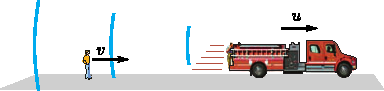
\includegraphics[width=0.95\linewidth]{figures/doppler-tilvik3.pdf}
    \vspace{0.3cm}
    \end{minipage}
    &
      Viðtakandi nálgast uppsprettu. \par Uppspretta fjarlægist viðtakanda.
    & 
      \begin{align*}
          f = \left( \frac{c + v}{c + u} \right)f_0
      \end{align*}
    \\ \hline
    \begin{minipage}{.4\textwidth}
    \vspace{0.3cm}
    \centering
      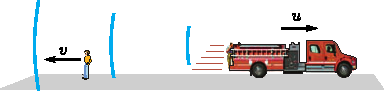
\includegraphics[width=0.95\linewidth]{figures/doppler-tilvik34.pdf}
    \vspace{0.3cm}
    \end{minipage}
    &
      Viðtakandi fjarlægist uppsprettu. \par Uppspretta fjarlægist viðtakanda.
    & 
      \begin{align*}
          f = \left( \frac{c - v}{c + u} \right)f_0
      \end{align*}
    \\ \hline
  \end{tabular}
  \caption{Allsherjarjafnan í öllum fjórum tilvikum.} \label{table:hverfi}
\end{table}

\newpage

\section{Eigintíðnir og eiginsveifluhættir}

Við höfðum séð að grunnlausnir bylgjujöfnunnar voru bylgjupúlsar af gerðinni $\psi(x,t) = A\sin(kx-\omega t + \varphi_0)$. Nú þurfum við að kafa aðeins dýpra í bylgjujöfnuna $\Ddot{\psi} = c^2\psi''$. Við athugum að:
\begin{tcolorbox}
\begin{theorem}
Lítum á bylgjujöfnuna $\Ddot{\psi} = c^2\psi''$. Með því að aðskilja bylgjufallið í rúmhnit og tímahnit $\psi(x,t) = f(x)g(t)$ þá sést að hvort hnit fyrir sig er á einfaldri sveifluhreyfingu:
\begin{align*}
    f'' = -k^2f, \hspace{1cm} \Ddot{g} = -\omega^2g.
\end{align*}
Þar sem $k$ er bylgjutalan og $\omega = kc$ er sveiflutíðnin.
\end{theorem}
\end{tcolorbox}

\textbf{Útleiðsla:} Við aðskiljum bylgjufallið í rúmhnit og tímahnit, $\psi(x,t) = f(x)g(t)$. Við höfum þá að:
\begin{align*}
    \Ddot{\psi} = c^2 \psi'' \implies f\Ddot{g} = c^2f'' g \implies \frac{1}{c^2} \frac{\Ddot{g}}{g} = \frac{f''}{f}
\end{align*}
En vinstri hliðin er einungis fall af $t$ og hægri hliðin er einungis fall af $x$. En þar með getum við ályktað að báðar hliðarnar verða að vera fastar! Þar með er til neikvæður fasti $-k^2$ (það er ekki augljóst að fastinn þurfi að vera neikvæður en ef maður gerir ráð fyrir að fastinn sé núll eða jákvæður þá fæst mótsögn!). Fastinn $k$ mun síðan reynast vera bylgjutalan! Við höfum þá að:
\begin{align*}
    \frac{1}{c^2} \frac{\Ddot{g}}{g} = -k^2, \hspace{2cm} \frac{f''}{f} = -k^2.
\end{align*}
Sem við getum umritað sem:
\begin{align*}
    \Ddot{g} = -(kc)^2g, \hspace{2cm} f'' = -k^2 f
\end{align*}
En þetta eru jöfnur fyrir tvær (mismunandi) einfaldar sveifluhreyfingar! Við ályktum því að:
\begin{align*}
    g(t) = \alpha \cos(kct + \beta), \hspace{1cm} f(x) = \gamma \sin(kx + \delta).
\end{align*}
Þar sem $\alpha, \beta, \gamma$ og $\delta$ er fastar sem ákvarðast út frá upphafsskilyrðunum. En þar með höfum við sýnt að:
\begin{align*}
\psi(x,t) = f(x)g(t) = \alpha \gamma \sin(kx + \delta) \cos(kct + \beta)
\end{align*}
Við notum síðan liðunarreglur hornafalla, $2\sin(u)\cos(v) = \sin(u+v) + \sin(u-v)$ til þess að fá:
\begin{align*}
    \psi(x,t) = A\sin(kx+kct + \phi) + A\sin(kx-kct + \varphi)
\end{align*}
Þar sem við höfum skilgreint nýja fasta $A = \frac{\alpha \gamma}{2}$, $\phi = \delta + \beta$ og $\varphi = \delta - \beta$. Ef við skilgreinum að lokum sveiflutíðnina sem $\omega = kc$ þá höfum við sýnt að grunnlausnirnar eru gefnar með
\begin{align*}
    \psi(x,t) = A\sin(kx + \omega t + \phi) + A\sin(kx - \omega t + \varphi). \qedhere
\end{align*}

Á þessum tímapunkti er hugsanlega vert að minnast á það að við segjum að $\psi_V(x,t) = A\sin(kx+\omega t + \phi)$ sé staðbylgja sem ferðast til vinstri en að $\psi_H(x,t) = A\sin(kx - \omega t + \varphi)$ sé staðbylgja sem ferðast til hægri (sjá bls. 100-102 í grænu bókinni til skýringar fyrir formerkið). 

\begin{tcolorbox}
\begin{definition}
Við segjum að jaðarskilyrði séu
\begin{enumerate}[label = \textbf{(\roman*)}]
    \item \textbf{Dirichlet} eða \textbf{lokuð} jaðarskilyrði ef $\psi(0,t) = \psi(\ell,t) = 0$.
    \item \textbf{Neumann} eða \textbf{opin} jaðarskilyrði ef $\psi'(0,t) = \psi'(\ell,t) = 0$.
    \item \textbf{Blönduð} jaðarskilyrði ef annar endinn hefur Neumann jaðarskilyrði og hinn endinn hefur Dirichlet jaðarskilyrði, þ.e.~$\psi(0,t) = \psi'(\ell,t) = 0$ eða $\psi'(0,t) = \psi(\ell,t) = 0$. 
\end{enumerate}
\end{definition}
\end{tcolorbox}

Við sjáum að jaðarskilyrðin eru í rauninni bara skilyrði sem við setjum á rúmhnitið af bylgjufallinu. Það segir til um það til dæmis hvort að strengur sé festur í báða enda (gítarstrengur) eða hvort að annar endirinn sé laus (blönduð jaðarskilyrði) eða hvort að þetta sé eins og opin pípa sem við blásum í gegnum (opin jaðarskilyrði. Þau eru semsagt rúmfræðilegar skorður sem að hluturinn sem við erum að skoða hefur. Það kemur í ljós að aðeins út frá því hver jaðarskilyrði strengsins eru þá getum við vitað hvernig hann mun sveiflast (og þar með hvaða tóna hann mun gefa frá sér).


\begin{tcolorbox}
\begin{theorem}
Annað hvort Dirichlet eða Neumann jaðarskilyrði.
\begin{align*}
    \lambda_n = \frac{2\ell}{n}, \hspace{1cm} f_n = nf_1, \hspace{2cm} n \in \Z_+.
\end{align*}
\end{theorem}
\end{tcolorbox}

\textbf{Útleiðsla:} Við höfðum sýnt að rúmhnitið fyrir bylgjufallið var: $f(x) = \gamma \sin(kx + \delta)$. Við athugum síðan að $\psi(0,t) = \psi(\ell,t) = 0$ er jafngilt því að $f(0) = f(\ell) = 0$. En þá höfum við að:
\begin{align*}
    f(0) = 0 \implies \gamma \sin(k\cdot 0 + \delta ) = 0 \implies \gamma \sin(\delta) = 0 \implies \delta = 0
\end{align*}
En þar með er $f(x) = \gamma \sin(kx)$. Við athugum síðan að:
\begin{align*}
    f(\ell) = 0 \implies \gamma \sin(k\ell) = 0 \implies k\ell = n\pi
\end{align*}
En þar með höfum við sýnt að $k = \frac{n\pi}{\ell}$. En það þýðir einmitt að $\lambda = \frac{2\pi}{k} = \frac{2\ell}{n}$. Við setjum síðan merkimiða $n$ á bylgjulengdina til þess að minna okkur á að þetta er háð heiltölunni $n$. Við athugum síðan að tilheyrandi tíðni er þá fundin með:
\begin{align*}
    f_n = \frac{c}{\lambda_n} = n \frac{c}{2\ell} = n \frac{c}{\lambda_1} = nf_1.
\end{align*}

Fyrir Neumann skilyrðin þá höfum við að $f'(x) = \gamma k \cos(k\ell + \delta)$ og þá
\begin{align*}
    f'(0) = 0 \implies \gamma k \cos(\delta) = 0 \implies \delta = \pm \frac{\pi}{2}. 
\end{align*}
En það er jafngilt því að $f'(x) = \gamma k \sin(k\ell)$ og þá fæst með sömu reikningum og áðan að eigintíðnirnar og eiginbylgjulengdirnar verða eins og fyrir Dirichlet skilyrðið.

\qed

\begin{tcolorbox}
\begin{theorem}
Blönduð, hálf-opin jaðarskilyrði
\begin{align*}
    \lambda_n = \frac{4\ell}{2n-1}, \hspace{1cm} f_n = (2n-1)f_1, \hspace{2cm} n \in \Z_+.
\end{align*}
\end{theorem}
\end{tcolorbox}

\textbf{Útleiðsla:} Ef $f(0) = 0$ þá höfum við eins og áður að þá sé $\delta = 0$ svo $f(x) = \gamma \sin(kx)$. Síðan athugum við að $f'(x) = \gamma k \cos(kx)$ og þá höfum við að:
\begin{align*}
    f'(\ell) = 0 \implies \gamma k \cos(k\ell) = 0 \implies k \ell = -\frac{\pi}{2} + n\pi \implies k = \frac{(2n-1)\pi}{2\ell}
\end{align*}
(Eina ástæðan fyrir að við veljum $-\frac{\pi}{2}$ en ekki $\frac{\pi}{2}$ er til þess að $n \in \Z_+$ en ekki $n \in \N$ í loksvarinu). En þar með höfum við að:
\begin{align*}
    \lambda_n = \frac{2\pi}{k} = \frac{4\ell}{2n-1}, \hspace{0.8cm} \text{sem gefur þá að} \hspace{0.8cm} f_n = \frac{c}{\lambda_n} = (2n-1) \frac{c}{4\ell} = (2n-1) \frac{c}{\lambda_1} = (2n-1)f_1.
\end{align*}

\qed

\begin{tcolorbox}
\begin{definition}
Tíðnirnar $f_n$ sem ákvarðast af jaðarskilyrðunum kallast \textbf{eigintíðnir} strengsins. Við segjum að $f_1$ sé \textbf{grunntónn} (eða fyrsti yfirtónn) strengsins og að $f_n$ sé \textbf{$\bm{n}$-ti yfirtónn} hans.
\end{definition}
\end{tcolorbox}

Ef ykkur finnst þetta vera svolítið flókið þá þurfið þið ekki að hafa neinar áhyggjur! Það er líka til einföld rúmfræðileg leið til þess að sjá þetta! Sem við munum nú skoða:

\begin{comment}
\begin{figure}[H]
    \centering
    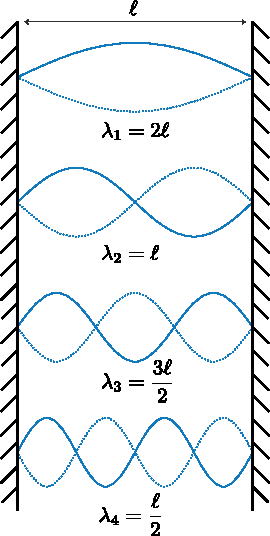
\includegraphics{figures/stadbylgjur.pdf}
    \caption{Strengur sem uppfyllir Dirichlet jaðarskilyrði og er festur í báða enda.}
    \label{fig:my_label}
\end{figure}
\end{comment}

\begin{figure}[H]
    \centering
    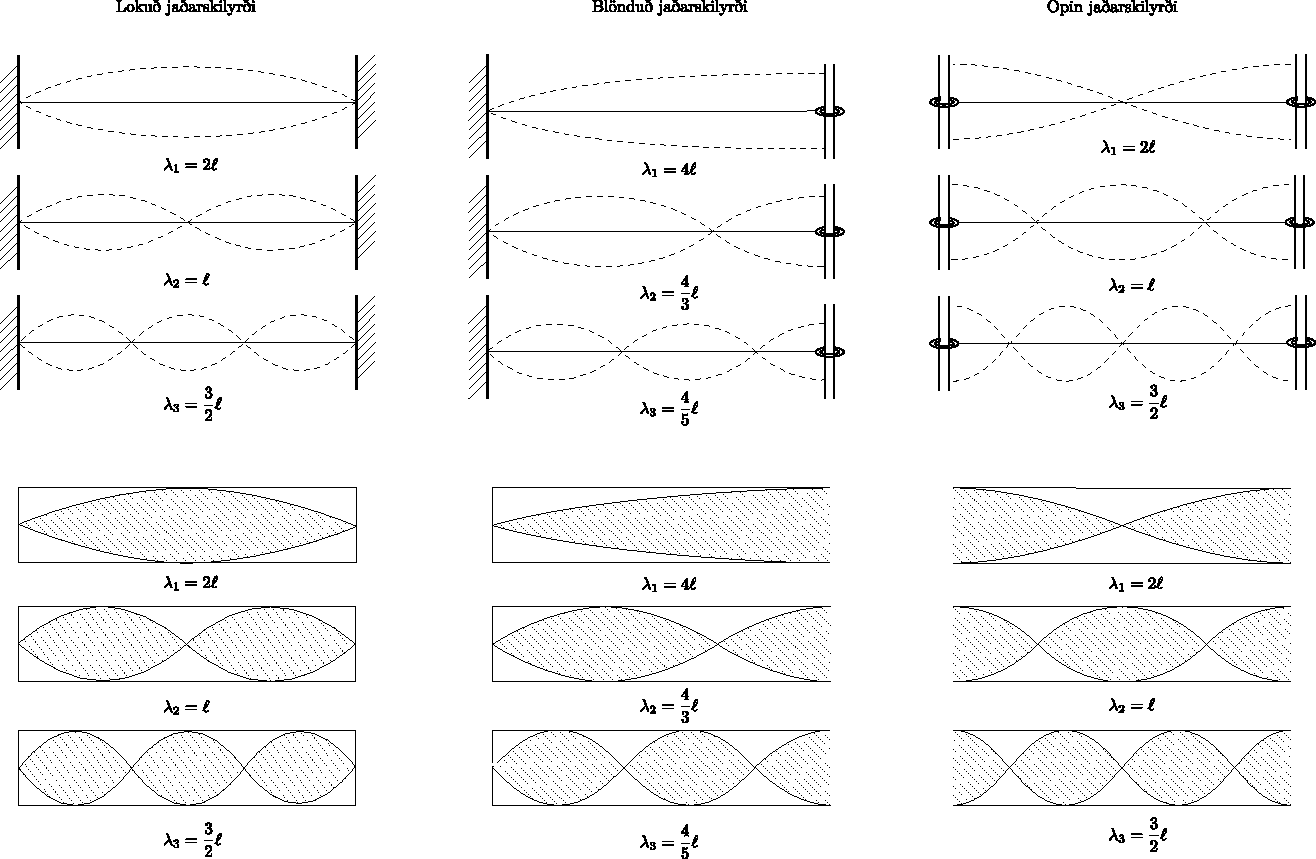
\includegraphics[width = \textwidth]{figures/neumann-stadbylgjurs.pdf}
    \caption{Fyrstu þrír eiginsveifluhættirnir fyrir mismunandi jaðarskilyrði.}
    \label{fig:eiginsveiflur}
\end{figure}

Að lokum minnumst við á tengslin milli staðbylgjunnar á strengnum og hljóðbylgjunnar sem hún myndar:

\begin{figure}[H]
    \centering
    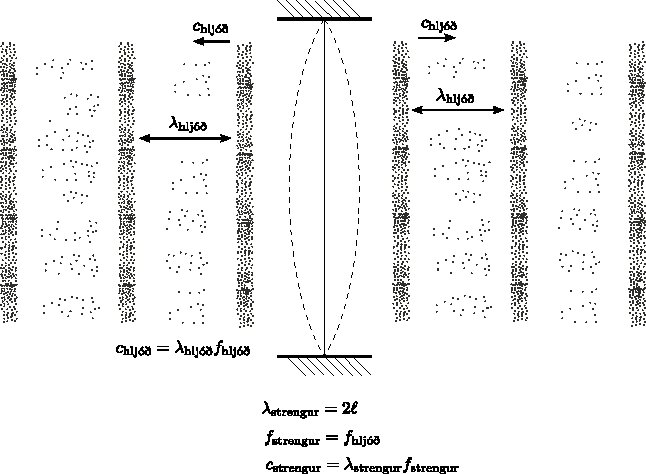
\includegraphics{figures/hljodbylgja-strengur.pdf}
    \label{fig:my_label}
    \caption{Tengslin milli staðbylgjunnar á strengnum og hljóðbylgjunnar sem sveifla strengsins myndar.}
\end{figure}


\section{Bylgjusamliðun}

\begin{tcolorbox}
\begin{theorem}
Hugsum okkur að við höfum tvær samfasa bylgjuuppsprettur í fjarlægð $d$ frá hvor annarri sem senda út eins bylgjur með útslag $A$, tíðni $f$ og bylgjulengd $\lambda$. Skoðum einhvern punkt, $P$, sem er þannig að önnur uppsprettan er í fjarlægð $r_1$ frá punktinum og hin uppsprettan er í fjarlægð $r_2$ frá punktinum.
\begin{figure}[H]
    \centering
    \vspace{-0.5cm}
    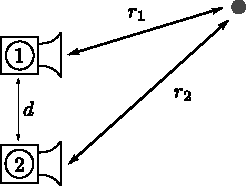
\includegraphics{figures/hatalari-dist.pdf}
\end{figure}
Þá er samliðunarbylgjan sem athugandi í punkti $P$ greinir gefin með:
\begin{align*} 
A\sin(kr_1-\omega t) + A\sin(kr_2 - \omega t) = 2A\cos(\frac{1}{2}k\Delta r)\sin(\frac{1}{2}k(r_1+r_2)-\omega t).
\end{align*}
Sér í lagi þá mun athugandinn heyra fullkomlega styrkjandi/eyðandi bylgjusamliðun í punkti $P$ ef:
\begin{align*}
    \Delta r = \begin{cases}
    n \lambda \hspace{2.8cm} \text{(styrkjandi bylgjusamliðun)} \\
    \left(n+\frac{1}{2}\right)\lambda \hspace{1.8cm} \text{(eyðandi bylgjusamliðun)}
    \end{cases},\hspace{1cm} n \in \N.
\end{align*}
\end{theorem}
\end{tcolorbox}

\textbf{Útleiðsla:} Skoðum samliðunarbylgjuna í punktinum $P$ en hún er gefin með:
\begin{align*}
    \psi_{\text{P}} = \psi_1 + \psi_2 = A \sin(k r_1 - \omega t) +  A \sin(k r_2 - \omega t)
\end{align*}
Með því að nota þáttunarreglur hornafalla (sjá bls. 68.~í grænu bókinni):
\begin{align*}
    \sin(s) + \sin(t) = 2\sin(\frac{s+t}{2})\cos(\frac{s-t}{2}),
\end{align*}
fæst að:
\begin{align*}
    \psi &= A \sin(k r_1 - \omega t) +  A \sin(k r_2 - \omega t) \\
    &= 2A\sin(\frac{\left(kr_1 - \omega t\right) + \left(k r_2 -\omega t\right)}{2})\cos(\frac{\left( k r_1 - \omega t \right) - \left( kr_2 - \omega t \right)}{2}) \\
    &= 2A\cos(\frac{1}{2}k\Delta r)\sin(\frac{1}{2}k(r_1+r_2)-\omega t).
\end{align*}
Við sjáum að samliðunarbylgjan hegðar sér eins og bylgja með fast útslag $B = 2A\cos(\frac{1}{2}k\Delta r)$, tíðni $f$ og bylgjulengd $\lambda$, sem rita mætti sem $\psi = B\sin(kr - \omega t)$ þar sem $r =  \frac{r_1 + r_2}{2}$ er meðalfjarlægðin frá hátölurunum. En þá fæst fullkomlega styrkjandi bylgjusamliðun $B = 2A$ ef:
\begin{align*}
    \cos(\frac{1}{2}k\Delta r) = 1 \implies \frac{1}{2}k\Delta r = n\pi \implies \Delta r = \frac{2n\pi}{k} = n\lambda.
\end{align*}
En fullkomlega eyðandi bylgjusamliðun $B = 0$ ef:
\begin{align*}
    \cos(\frac{1}{2}k\Delta r) = 0 \implies \frac{1}{2}k\Delta r = \frac{\pi}{2} + n\pi = (2n+1)\frac{\pi}{2} \implies \Delta r = (2n +1)\frac{\pi}{k} = \left(n + \frac{1}{2}\right)\lambda.
\end{align*}
Almennt segjum við að samliðun sé \textbf{styrkjandi} ef $B > A$ og \textbf{eyðandi} ef $B < A$. \qed


\section{Hviður}


\begin{tcolorbox}
\begin{theorem}
Hugsum okkur að við höfum tvær samfasa bylgjuuppsprettur í fjarlægð $d$ frá hvor annarri sem senda út bylgjur með sama útslag $A$ en mismunandi tíðnir $f_1$ og $f_2$. Skoðum einhvern punkt, $P$, sem er þannig að önnur uppsprettan er í fjarlægð $r_1$ frá punktinum og hin uppsprettan er í fjarlægð $r_2$ frá punktinum. Þá heyrir athugandi í punktinum $P$ samliðunarbylgju sem styrkist og eyðist með hviðutíðni:
\begin{align*}
    f_{\text{hviður}} = \Delta f = f_2 - f_1.
\end{align*}
\begin{figure}[H]
    \centering
    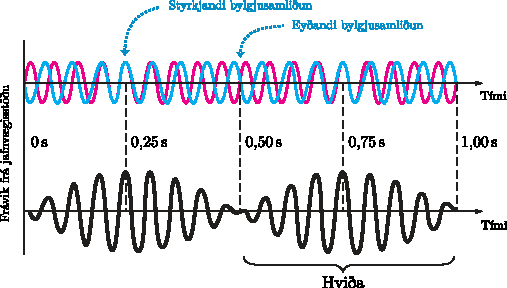
\includegraphics{figures/hvidur.pdf}
\end{figure}
\end{theorem}
\end{tcolorbox}

\textbf{Útleiðsla:} Skoðum samliðunarbylgjuna í punktinum $P$ en hún er gefin með:
\begin{align*}
    \psi_{_\text{P}} = \psi_1 + \psi_2 = A \sin(k_1 r_1 - \omega_1 t) +  A \sin(k_2 r_2 - \omega_2 t)
\end{align*}
Með því að nota þáttunarreglur hornafalla (sjá bls. 68.~í grænu bókinni):
\begin{align*}
    \sin(s) + \sin(t) = 2\sin(\frac{s+t}{2})\cos(\frac{s-t}{2}),
\end{align*}
fæst að:
\vspace{-0.75cm}
\begin{align*}
    \psi &= A \sin(k_1 r_1 - \omega t) +  A \sin(k_2 r_2 - \omega t) \\
    &= 2A\sin(\frac{\left(k_1r_1 - \omega_1 t\right) + \left(k_2 r_2 -\omega_2 t\right)}{2})\cos(\frac{\left( k r_1 - \omega_1 t \right) - \left( kr_2 - \omega_2 t \right)}{2}) \\
    &= 2A\cos(\frac{1}{2}\Delta(kr) - \frac{1}{2}\Delta \omega t)\sin(\frac{1}{2}(k_1r_1+k_2r_2)-\frac{1}{2}(\omega_1+\omega_2) t).
\end{align*}
Við munum því heyra hljóð með meðaltíðnina $f = \frac{1}{2}(f_1 + f_2)$. Hinsvegar þá mun mismunurinn í tíðnunum valda hviðutíðni sem eyðir og styrkir útslag hljóðbylgjunnar með jöfnum tímamismun. Við sjáum hér að ofan að ein hviða samsvarar hálfum sveiflutíma kósínusfallsins því ein hviða jafngildir því að kósínusinn fari frá því að vera núll, síðan einn og síðan aftur núll, en það er einmitt hálfur sveiflutími svo við höfum að:
\begin{align*}
    f_{\text{hviður}} = \frac{2}{T} = \frac{2}{\frac{2\pi}{\frac{1}{2}\Delta \omega}} = \Delta f.
\end{align*}
\qed


\newpage

\section{Tónlist (ítarefni)} 

\textit{Athugið: Ég hef aldrei lært tónfræði, svo takið þessum kafla með fyrirvara. Hinsvegar hefur meðhöfundur þessa kafla, Álfheiður Edda Sigurðardóttir, lært mannganginn í tónfræði. Ef þið hafið einhverjar ábendingar, sama hversu smávægilegar, um hvernig mætti orða hlutina betur í samræmi við það sem tíðkast í tónfræði þá megið þið endilega senda okkur ábendingar þess varðandi! Ath: tónbil = k}


Við skulum byrja á því að setja fram nóturnar og tilheyrandi tíðnir þeirra hér fyrir neðan:


\begin{table}[H]
\begin{center}
\begin{tabular}{|c|c|}
\hline
\textbf{Nóta} & \textbf{Tíðni [Hz]} \\
\hline
\hline
$C_0$ & $\SI{16.35}{}$ \\
$D^\flat_0$ & $\SI{17.32}{}$ \\
$D_0$ & $\SI{18,35}{}$ \\
$E^\flat_0$ & $\SI{19,45}{}$ \\
$E_0$ & $\SI{20.60}{}$ \\
$F_0$ & $\SI{21,83}{}$ \\
$G^\flat_0$ & $\SI{23,12}{}$ \\
$G_0$ & $\SI{24,50}{}$ \\
$A^\flat_0$ & $\SI{25,96}{}$ \\
$A_0$ & $\SI{27,50}{}$ \\
$B^\flat_0$ & $\SI{29,14}{}$ \\
$B_0$ & $\SI{30,87}{}$ \\
\hline
\end{tabular}
\quad
\begin{tabular}{|c|c|}
\hline
\textbf{Nóta} & \textbf{Tíðni [Hz]} \\
\hline
\hline
$C_1$ & $\SI{32.70}{}$ \\
$D^\flat_1$ & $\SI{34.65}{}$ \\
$D_1$ & $\SI{36.71}{}$ \\
$E^\flat_1$ & $\SI{38.89}{}$ \\
$E_1$ & $\SI{41.20}{}$ \\
$F_1$ & $\SI{43.65}{}$ \\
$G^\flat_1$ & $\SI{46.25}{}$ \\
$G_1$ & $\SI{49.00}{}$ \\
$A^\flat_1$ & $\SI{51.91}{}$ \\
$A_1$ & $\SI{55.00}{}$ \\
$B^\flat_1$ & $\SI{58.27}{}$ \\
$B_1$ & $\SI{61.74}{}$ \\
\hline
\end{tabular}
\quad
\begin{tabular}{|c|c|}
\hline
\textbf{Nóta} & \textbf{Tíðni [Hz]} \\
\hline
\hline
$C_2$ & $\SI{65.41}{}$ \\
$D^\flat_2$ & $\SI{69.30}{}$ \\
$D_2$ & $\SI{73.42}{}$ \\
$E^\flat_2$ & $\SI{77.78}{}$ \\
$E_2$ & $\SI{82.41}{}$ \\
$F_2$ & $\SI{87.31}{}$ \\
$G^\flat_2$ & $\SI{92.50}{}$ \\
$G_2$ & $\SI{98.00}{}$ \\
$A^\flat_2$ & $\SI{103.83}{}$ \\
$A_2$ & $\SI{110.00}{}$ \\
$B^\flat_2$ & $\SI{116.54}{}$ \\
$B_2$ & $\SI{123.47}{}$ \\
\hline
\end{tabular}
\quad
\begin{tabular}{|c|c|}
\hline
\textbf{Nóta} & \textbf{Tíðni [Hz]} \\
\hline
\hline
$C_3$ & $\SI{130.81}{}$ \\
$D^\flat_3$ & $\SI{138.59}{}$ \\
$D_3$ & $\SI{146.83}{}$ \\
$E^\flat_3$ & $\SI{155.56}{}$ \\
$E_3$ & $\SI{164.81}{}$ \\
$F_3$ & $\SI{174.61}{}$ \\
$G^\flat_3$ & $\SI{185.00}{}$ \\
$G_3$ & $\SI{196.00}{}$ \\
$A^\flat_3$ & $\SI{207.65}{}$ \\
$A_3$ & $\SI{220.00}{}$ \\
$B^\flat_3$ & $\SI{233.08}{}$ \\
$B_3$ & $\SI{246.94}{}$ \\
\hline
\end{tabular}
\label{tafla:las}
\end{center}
\end{table}

\begin{table}[H]
\begin{center}
\begin{tabular}{|c|c|}
\hline
\textbf{Nóta} & \textbf{Tíðni [Hz]} \\
\hline
\hline
$C_4$ & $\SI{261.63}{}$ \\
$D^\flat_4$ & $\SI{277.18}{}$ \\
$D_4$ & $\SI{293.66}{}$ \\
$E^\flat_4$ & $\SI{311.13}{}$ \\
$E_4$ & $\SI{329.63}{}$ \\
$F_4$ & $\SI{349.23}{}$ \\
$G^\flat_4$ & $\SI{369.99}{}$ \\
$G_4$ & $\SI{392.00}{}$ \\
$A^\flat_4$ & $\SI{415.30}{}$ \\
$A_4$ & $\SI{440.00}{}$ \\
$B^\flat_4$ & $\SI{466.16}{}$ \\
$B_4$ & $\SI{493.88}{}$ \\
\hline
\end{tabular}
\quad
\begin{tabular}{|c|c|}
\hline
\textbf{Nóta} & \textbf{Tíðni [Hz]} \\
\hline
\hline
$C_5$ & $\SI{523.25}{}$ \\
$D^\flat_5$ & $\SI{554.37}{}$ \\
$D_5$ & $\SI{587.33}{}$ \\
$E^\flat_5$ & $\SI{622.25}{}$ \\
$E_5$ & $\SI{659.25}{}$ \\
$F_5$ & $\SI{698.46}{}$ \\
$G^\flat_5$ & $\SI{739.99}{}$ \\
$G_5$ & $\SI{783.99}{}$ \\
$A^\flat_5$ & $\SI{830.61}{}$ \\
$A_5$ & $\SI{880.00}{}$ \\
$B^\flat_5$ & $\SI{932.33}{}$ \\
$B_5$ & $\SI{987.77}{}$ \\
\hline
\end{tabular}
\quad
\begin{tabular}{|c|c|}
\hline
\textbf{Nóta} & \textbf{Tíðni [Hz]} \\
\hline
\hline
$C_6$ & $\SI{1046.50}{}$ \\
$D^\flat_6$ & $\SI{1108.73}{}$ \\
$D_6$ & $\SI{1174.66}{}$ \\
$E^\flat_6$ & $\SI{1244.51}{}$ \\
$E_6$ & $\SI{1318.51}{}$ \\
$F_6$ & $\SI{1396.91}{}$ \\
$G^\flat_6$ & $\SI{1479.98}{}$ \\
$G_6$ & $\SI{1567.98}{}$ \\
$A^\flat_6$ & $\SI{1661.22}{}$ \\
$A_6$ & $\SI{1760.00}{}$ \\
$B^\flat_6$ & $\SI{1864.66}{}$ \\
$B_6$ & $\SI{1975.53}{}$ \\
\hline
\end{tabular}
\quad
\begin{tabular}{|c|c|}
\hline
\textbf{Nóta} & \textbf{Tíðni [Hz]} \\
\hline
\hline
$C_7$ & $\SI{2093.00}{}$ \\
$D^\flat_7$ & $\SI{2217.46}{}$ \\
$D_7$ & $\SI{2349.32}{}$ \\
$E^\flat_7$ & $\SI{2489.02}{}$ \\
$E_7$ & $\SI{2637.02}{}$ \\
$F_7$ & $\SI{2793.83}{}$ \\
$G^\flat_7$ & $\SI{2959.96}{}$ \\
$G_7$ & $\SI{3135.96}{}$ \\
$A^\flat_7$ & $\SI{3322.44}{}$ \\
$A_7$ & $\SI{3520.00}{}$ \\
$B^\flat_7$ & $\SI{3729.31}{}$ \\
$B_7$ & $\SI{3951.07}{}$ \\
\hline
\end{tabular}
\end{center}
\end{table}

Ef við skoðum síðan hvað gerist við ákveðinn bókstaf þegar $n$ hækkar. Þá er:

\begin{table}[H]
    \centering
\begin{tabular}{|c|c|c|c|c|c|c|c|c|c|}
\hline
\textbf{Nóta} & $A_0$ & $A_1$ & $A_2$ & $A_3$ & $A_4$ & $A_5$ & $A_6$ & $A_7$ \\
\hline
\textbf{Tíðni [Hz]} & $\SI{27.50}{}$ & $\SI{55}{}$ & $\SI{110}{}$ & $\SI{220}{}$ & $\SI{440}{}$ & $\SI{880}{}$ & $\SI{1760}{}$ & $\SI{3520}{}$ \\
\hline
\end{tabular}
\end{table}

Það er að segja við sjáum að tíðnin tvöfaldast í hvert skipti sem að við hækkum $n$. Sama gildir um alla hina tónana í töflunni. Við höfum semsagt eftirfarandi lögmál:

\begin{tcolorbox}
\begin{theorem}
Látum $f_{C_n}$ tákna tíðni tónsins $C_n$ og $n$ tákna hæðirnar á tónstigunum. Þá gildir að:
\begin{align*}
    f_{C_n} = 2^{n}f_{C_0}, \hspace{0.5cm} \text{þar sem $f_{C_0} = \SI{16.35}{Hz}$.}
\end{align*}
Sambærileg niðurstaða gildir fyrir alla hina tólf tónana.
\end{theorem}
\end{tcolorbox}

\newpage

Við skoðum núna annan merkilegan eiginleika sem að tónarnir hafa. Við skoðum nú graf af tíðnum tónanna, $f$ sem fall af nótunum, en þá þurfum við fyrst að úthluta tónunum einhverri tölu (við getum ekki gert gröf af bókstöfum!). Það er því eðlilegast að raða þeim bara í stærðarröð þannig að $C_0 = 1$, $D^\flat_0 = 2$, $D_0 = 3$, \ldots, $A^\flat_2 = 35$, \ldots, $G_6 = 80$, \ldots, $B_7 = 96$. Þá fáum við eftirfarandi veldisvísisgraf:

\begin{figure}[H]
    \centering
    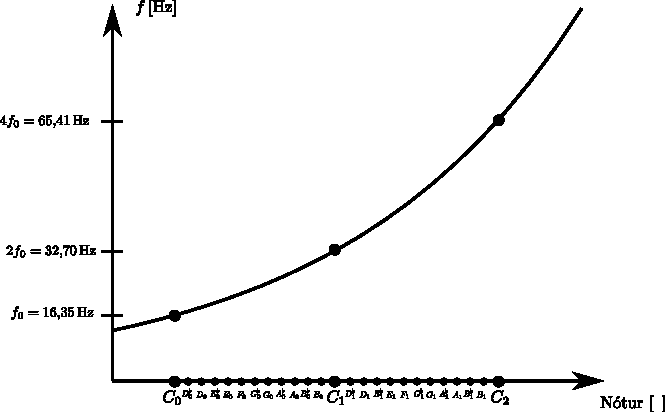
\includegraphics{figures/music-notes.pdf}
    \caption{Graf sem sýnir hvernig að tíðnin vex með veldisfalli sem fall af nótunum.}
    \label{fig:my_label}
\end{figure}
En við sjáum þar með að í hverju þrepi tónstigans á hæð $n$ þá hækkar tíðnin um $2^{\frac{1}{12}}$. Í hverri hæð eru síðan $12$ tónar svo að þetta passar við niðurstöðuna sem við sáum áðan að þegar við hækkum um heila tónhæð þá tvöfaldast tíðnin því þá erum við að hækka um $k = 12$ þrep og þar með $\left(2^{\frac{1}{12}}\right)^{12} = 2$.

\begin{tcolorbox}
\begin{theorem}
Látum $k$ tákna hvert þrep í tónstiganum ($k = 1$ fyrir $C_0$ upp í $k = \SI{96}{}$ fyrir $B_7$). Þá gildir að tíðnin, $f_k$, $k$ þrepum ofar í tónstiganum er gefin með:
\begin{align*}
    f_k = 2^{\frac{k}{12}} f_0, \hspace{1cm} \text{þar sem $f_0 = \SI{16.35}{Hz}$.}
\end{align*}
\end{theorem}
\end{tcolorbox}

Til dæmis getum við þá athugað að við höfum að $A_4$ er $k = 57$ þrepum fyrir ofan $C_0$ svo við fáum að:
\begin{align*}
    f_{57} = 2^{\frac{57}{12}} f_0 = \SI{440}{Hz}
\end{align*}
Sem er einmitt tíðnin sem við tengjum við nótuna $A_4$. Það er hinsvegar óþæginlegt að þurfa að burðast um með svona háar tölur og telja svona hátt upp svo venjulega endurskilgreinir tónlistarfólk skalan í kringum $A_4$ (því það er svo gott sem í miðjunni á öllum þeim nótum sem maður þarf að nota). Þá gildir sama lögmál nema núna er:
\begin{align*}
    f_k = 2^{\frac{k}{12}}f_0, \hspace{1cm} \text{þar sem $f_0 = \SI{440}{Hz}$,}
\end{align*}
Þar sem $k$ er neikvætt ef þrepið er fyrir neðan $A_4$ og jákvætt ef þrepið er fyrir ofan $A_4$. Þannig myndum við til dæmis geta fundið tíðnina á nótunni $D^\flat_0$ sem er $k = -8$ þrepum fyrir neðan $A_4$. En hún hefur tíðni:
\begin{align*}
    f_{D^\flat_4} = 2^{-\frac{8}{12}} f_0 = \SI{277.18}{Hz}.
\end{align*}
En þetta þýðir að það er einmitt nóg að velja einn tón og stilla alla hina tónana í samræmi við það.


\newpage 

\section{Chladni platan (ítarefni)}

Að lokum skulum við aðeins fjalla um það hvað gerist þegar við höfum bylgjujöfnuna í hærri víddum. Í tveim rúmvíddum þá verður bylgjujafnan:

\begin{align*}
    \pdv[2]{\psi}{t} = c^2\left( \pdv[2]{\psi}{x} + \pdv[2]{\psi}{y} \right)
\end{align*}
Þar sem $c = \sqrt{\frac{S}{\sigma}}$ er bylgjuhraðinn, $S$ er yfirborðsspenna plötunnar og $\sigma$ er massi hennar á flatareiningu. Við höfum að lausnirnar eru gefnar með:
\begin{align*}
    \psi(x,y,t) = A\sin( kx + hy - \omega t + \varphi).
\end{align*}
Þar sem $A$ er útslag bylgjunnar, $\smqty(k \\ h)$ er bylgjuvigurinn, $\omega$ er sveiflutíðnin og $\varphi$ er fasahornið. Við höfum síðan að $\omega^2 = c^2\left(k^2 + h^2 \right)$. Ef við skoðum rétthyrningslaga Chladni-plötu með hliðarlengdir $\ell$ sem er fest í miðjunni þá gefa jaðarskilyrðin okkur að eiginsveifluhættirnir ákvarðast af $k = \frac{n\pi}{\ell}$ og $h = \frac{m\pi}{\ell}$ þar sem $n,m \in \N$. Við fáum að eigintíðnirnar, $f_{nm}$, eru nú háðar bæði $n$ og $m$ og eru gefnar með:
\begin{align*}
    f_{nm} = \frac{c}{2\ell} \sqrt{n^2 + m^2}. 
\end{align*}
Ef við myndum strá sandi yfir plötuna og síðan leyfa henni að sveiflast þá væru þetta mynstrin sem við myndum sjá fyrir eiginsveifluhættina:

\begin{figure}[H]
    \centering
    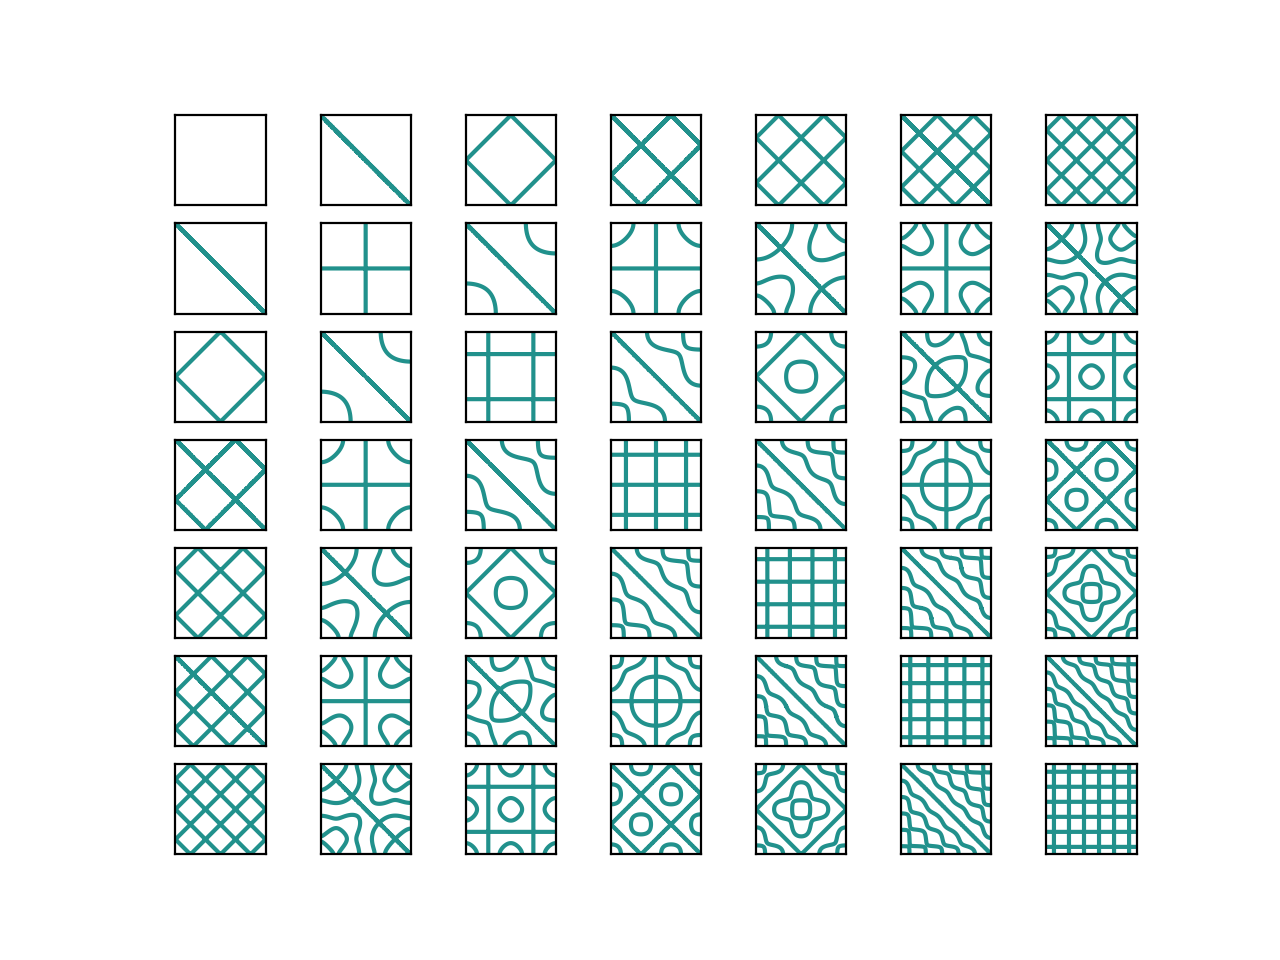
\includegraphics[width = \textwidth]{figures/chlad.png}
    \caption{Taflan sýnir eiginsveifluhátt $(n,m)$ fyrir Chladni plötuna. Efst til vinstri er eiginsveifluhátturinn  $(0,0)$ og neðst til hægri er eiginsveifluhátturinn $(6,6)$. Gildin á $n$ vaxa til hægri en gildin á $m$ vaxa niður.}
    \label{fig:chlad}
\end{figure}

\begin{comment}
Að lokum setjum við fram eitt athyglisvert varðveislulögmál sem segir að hlutföllin á milli tíðna tónanna eru varðveitt í hverri hæð tónstigans.

\begin{tcolorbox}
\begin{theorem}
Hlutföllin milli tveggja tóna í tónstiganum eru varðveitt þ.e.a.s.~
\begin{align*}
    \frac{C_n}{D_n} = \frac{C_0}{D_0}.
\end{align*}
\end{theorem}
\end{tcolorbox}
\end{comment}






\begin{comment}
\begin{table}[H]
\begin{center}
\begin{tabular}{|c|l|}
\hline
\textbf{Skynstyrkur hávaðans} & \textbf{Skólabókardæmi} \\
\hline
$\SI{0}{dB}$ & Lægsta hljóð sem mannseyrað getur greint. \\
$\SI{10}{dB}$ & Andardráttur \\
$p = mv $ & Hvísl \\
$K = \frac{1}{2}mv^2$ & Bókasafn \\
$W = Fd\cos\gamma$ &  \\
\hline
\end{tabular}
\caption{Hliðstæðar jöfnur fyrir línulega hreyfingu og snúningshreyfingu.}
\label{tafla:laddi}
\end{center}
\end{table}
\end{comment}

\newpage

\section{Dæmi}

\subsection*{Staðbylgjur á streng}

\begin{tcolorbox}
Við skoðuðum í þessum kafla staðbylgjur sem ferðast eftir streng sem hefur massa $m$ og lengd $\ell$. Við skilgreindum þá línulegan þéttleika vírsins sem stærðina $\mu := \frac{m}{\ell}$. Ef við strekkjum vírinn með togkrafti $T$ þá munu bylgjurnar ferðast með hraða $v = \sqrt{\frac{T}{\mu}} = \sqrt{\frac{T \ell }{m}}$ meðfram strengnum.
\end{tcolorbox}

\begin{enumerate}[label = \textbf{Dæmi \thechapter.\arabic*.}]

\item  \textit{(RK 16.1.)} Staðbylgja berst eftir streng með hraðanum $v = \SI{200}{m/s}$. Strengurinn hefur línulegan þéttleika $\mu = \SI{1.3e-4}{kg/m}$. \begin{enumerate*}[label = \textbf{(\alph*)}]
    \item Hver er togkrafturinn í strengnum?
    \item Hver væri hraði bylgjunnar ef togkrafturinn væri helmingi minni?
\end{enumerate*}

\item  \textit{(RK 16.2.)} Þegar togkrafturinn í streng nokkrum er $\SI{75}{N}$ þá ferðast staðbylgjur á strengnum með hraða $\SI{150}{m/s}$. Hver þyrfti togkrafturinn í strengnum að vera til þess að bylgjurnar bærust með hraða $\SI{180}{m/s}$ eftir strengnum?

\item \textit{(RK 16.3.)} Strengur með massa $\SI{25}{g}$ er strekktur með togkrafti $\SI{20}{N}$. Hversu langur er strengurinn ef það tekur bylgjupúls $\SI{50}{ms}$ að fara frá einum enda strengsins til hins endans?

\begin{minipage}{\linewidth}

\begin{wrapfigure}{r}{1.5in}
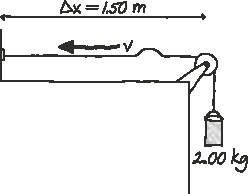
\includegraphics[width = 1.5in]{figures/waveslington.pdf}
\end{wrapfigure}

\item Á myndinni hér til hægri má sjá $\SI{2.00}{m}$ langan málmvír sem er festur við $\SI{2.00}{kg}$ lóð yfir núningslausa, massalausa trissu. Málmvírinn er festur við vegg í hinn endann þannig að $\Delta x = \SI{1.50}{m}$ af málmvírnum hanga yfir borðinu milli veggsins og trissunnar. Nú plokkum við strenginn þannig að staðbylgja byrjar að ferðast meðfram strengnum. Með ofursnjallsímanum okkar tekst okkur að mæla tímann, $\Delta t = \SI{18.0}{ms}$ sem það tekur bylgjuna að ferðast frá trissunni og að veggnum. \begin{enumerate*}[label = \textbf{(\alph*)}]
    \item Hver er togkrafturinn í strengnum?
    \item Hver er hraði bylgjunnar?
    \item Hver er línulegur þéttleiki strengsins?
    \item Hver er massi strengsins?
\end{enumerate*}
\end{minipage}

\begin{minipage}{\linewidth}

\begin{wrapfigure}{r}{1.5in}
\vspace{-0.5cm}
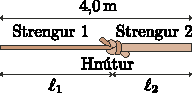
\includegraphics[width = 1.5in]{figures/strengur12.pdf}
\end{wrapfigure}

\item \textit{(RK 16.47.)} Strengur 1 á myndinni hér til hægri hefur lengd $\ell_1$ og línulegan þéttleika $\mu_1 = \SI{2.0}{g/m}$. Strengur 2 hefur lengd $\ell_2$ og línulegan þéttleika $\mu_2 = \SI{4.0}{g/m}$. Strengirnir eru festir við sitt hvorn vegginn og síðan bundnir saman með hnút. Eðlisfræðinemandi heldur í hnútinn og sveiflar hnútnum upp og niður í lóðrétta stefnu. Vegalengdin á milli veggjanna er $L = \ell_1 + \ell_2 = \SI{4.0}{m}$. Hver er lengdin á hvorum streng fyrir sig ef að staðbylgjurnar sem myndast við sveifluna lenda á veggjunum á sama tíma?
\end{minipage}

\begin{minipage}{\linewidth}
\begin{wrapfigure}{r}{1.5in}
\vspace{-1cm}
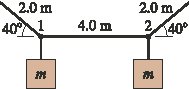
\includegraphics[width = 1.5in]{figures/hanger.pdf}
\end{wrapfigure}

\item \textit{(RK 16.58.)} Tveir jafnstórir massar $m$ hanga í stálvír með línulegan þéttleika $\mu = \SI{6.8}{g/m}$ eins og sést á myndinni hér til hægri. Hver er massinn $m$ ef það tekur staðbylgju $\SI{24.0}{ms}$ að ferðast frá punkti 1 í punkt 2?
\end{minipage}

\item Fiðlustrengir eru misþykkir (en úr sama efni) og þykkasti strengurinn hefur línulegan þéttleika $\mu_{1} = \SI{3.0}{g/m}$ en sá þynnsti hefur línulegan þéttleika $\mu_{2} = \SI{0.29}{g/m}$. Látum $r$ tákna geisla þunna strengsins og $R$ tákna geisla þykka strengsins. Ákvarðið hlutfallið $\frac{r}{R}$.


\begin{comment}
\begin{minipage}{\linewidth}

\begin{wrapfigure}{r}{1.5in}
\vspace{-0.5cm}
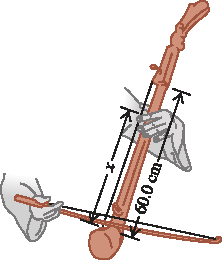
\includegraphics[width = 1.25in]{figures/fidla.pdf}
\end{wrapfigure}

\item Á strengjarhljóðfærinu sem sést á myndinni hér til hægri er lengd strengsins $\ell = \SI{60.0}{cm}$ og massi þessi hluta af strengnum er $\SI{1.99}{g}$. Þegar slegið er á strenginn heyrist nótan $A_4$ sem samsvarar $\SI{440}{Hz}$. 
\end{minipage}
\end{comment}

\end{enumerate}

\subsection*{Svör}

\begin{enumerate*}[label = \vspace{0.15cm} \textbf{(\arabic*)}]
  \item $T = \SI{5.2}{N}$, $v = \SI{140}{m/s}$.
  \item $T = \SI{110}{N}$.
  \item $\ell = \SI{2.0}{m}$.
  \item $T = \SI{19.6}{N}$, $v = \SI{83}{m/s}$, $\mu = \SI{2.8}{g/m}$, $m = \SI{5.6}{g}$.
  \item $\ell_1 = \SI{2.34}{m}$, $\ell_2 = \SI{1.66}{m}$.
  \item $m = \SI{16.1}{kg}$.
  \item $\frac{r}{R} = \SI{0.31}{}$.
\end{enumerate*}


\newpage 

\subsection*{Hreyfilýsingin}

\begin{tcolorbox}
Við sáum að hreyfilýsing staðbylgju var gefin með:
\begin{align*}
    \psi(x,t) = A\sin(kx - \omega t + \varphi_0)
\end{align*}
Þar sem $\omega = kc$ og $c$ er bylgjuhraði staðbylgjunnar í miðlinum sem hún berst í. Við segjum að $\omega = \frac{2\pi}{T} = 2\pi f$ sé sveiflutíðni bylgjunnar, $T$ sé sveiflutíminn og $f$ sé tíðni bylgjunnar. Ef $\lambda$ táknar bylgjulengd bylgjunnar (lengdin milli öldutoppa hennar) þá höfum við að bylgjutalan, $k$, er gefin með $k = \frac{2\pi}{\lambda}$. Fasamunurinn $\varphi_0$ og útslagið $A$ ákvarðast síðan af upphafsskilyrðunum.
\end{tcolorbox}

\begin{enumerate}[label = \textbf{Dæmi \thechapter.\arabic*.}]

\setcounter{enumi}{7}

\item \textit{(RK 16.10.)} Staðbylgja hefur sveiflutíðni $\SI{22}{rad/s}$ og bylgjulengd $\SI{7.0}{m}$. Hver er bylgjutala bylgjunnar og bylgjuhraði hennar?

\item \textit{(RK 16.11.)} Staðbylgja hefur bylgjuhraða \SI{287}{m/s} og bylgjutölu \SI{2.4}{rad/m}. Hver er bylgjulengd bylgjunnar og tíðni hennar?

\item \textit{(RK 16.13.)} Hreyfilýsing staðbylgju er gefin með $y(x,t) = \SI{0.025}{}\sin(\SI{1.8}{}x-66t)$ þar sem allar stærðir eru í SI-einingum. Hver er \begin{enumerate*}[label = \textbf{(\alph*)}]
    \item tíðnin
    \item bylgjulengdin
    \item bylgjuhraðinn?
\end{enumerate*}

\item Hreyfilýsing staðbylgju er gefin með $\psi(x,t) = \SI{6.0e-5}{}\cos( 1800 t - \SI{5.3}{}x)$ þar sem allar stærðir eru í SI-einingum. Hver er \begin{enumerate*}[label = \textbf{(\alph*)}]
    \item tíðnin
    \item bylgjulengdin
    \item bylgjuhraðinn?
\end{enumerate*}

\begin{minipage}{\linewidth}

\begin{wrapfigure}{r}{2.9in}
\vspace{-0.5cm}
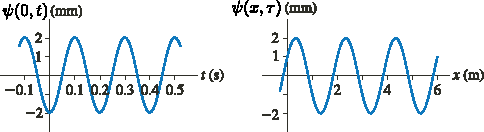
\includegraphics[width = 3in]{figures/both-at-the-same-time2.pdf}
\end{wrapfigure}

\item \textit{(RK 16.45.)} Lítum á gröfin hér til vinstri sem sýna graf af staðbylgju $\psi(x,t) = A\sin(kx-\omega t + \varphi_0)$. Vinstra grafið sýnir $\psi$ einungis sem fall af $t$ í staðsetningunni $x = \SI{0}{m}$. Hægra grafið sýnir $\psi$ einungis sem fall af $x$ við tíma $t = \tau$. Ákvarðið
\begin{enumerate*}[label = \textbf{(\alph*)}]
    \item Útslagið.
    \item Lotutímann.
    \item Tíðnina.
    \item Sveiflutíðnina.
    \item Fasahornið.
    \item Bylgjulengdina.
    \item Bylgjutöluna.
    \item Bylgjuhraðann.
    \item Tímann $\tau$.
\end{enumerate*}
\end{minipage}

\item \textit{(RK 16.19.)} Mannsaugað getur greint ljós með bylgjulengd frá \SI{380}{nm} (fjólublátt) upp í \SI{700}{nm} (rautt). Á hvaða tíðnibili eru þessar ljósbylgjur ef hraði ljóssins er $c = \SI{3.00e8}{m/s}$? 

\item \textit{(RK 16.20.)} \begin{enumerate*}[label = \textbf{(\alph*)}] \item Útvarpsstöðin FM957 heitir því nafni þar sem að hún sendir út allt efnið sitt með rafsegulbylgjum sem hafa tíðnina \SI{95.7}{MHz}. Hver er bylgjulengdin? \item Íslenska $\pi$-félagið ætlar að stofna útvarpsstöð sem sendir út allt efnið sitt með bylgjulengd $\lambda = \pi \si{m}$. Hvaða tíðni samsvarar það?
\end{enumerate*}
\end{enumerate}

\subsection*{Svör}

\begin{enumerate*}[label = \vspace{0.15cm} \textbf{(\arabic*)}]
    \setcounter{enumi}{7}
  \item $k = \SI{0.90}{rad/m}$, $c = \SI{25}{m/s}$.
  \item $\lambda = \SI{2.6}{m}$, $f = \SI{110}{Hz}$
  \item $f = \SI{10.5}{Hz}$, $\lambda = \SI{3.5}{m}$, $c = \SI{37}{m/s}$.
  \item $f = \SI{286}{Hz}$, $\lambda = \SI{1.19}{m}$, $c = \SI{340}{m/s}$.
  \item $A = \SI{2}{mm}$, $T = \SI{0.2}{s}$, $f = \SI{5}{Hz}$, $\omega = 10 \pi \si{rad/s}$, $\varphi_0 = -\frac{\pi}{2}$, $\lambda = \SI{2}{m}$, $k = \pi \si{rad/m}$, $c = \SI{10}{m/s}$, $\tau = \SI{67}{ms}$.
  \item $f \in [\SI{430}{THz}, \SI{790}{THz}]$.
  \item $\lambda = \SI{3.13}{m}$, $f = \SI{95.4}{MHz}$
\end{enumerate*}

\newpage

\subsection*{Hljóðstyrkur og hávaði}

\begin{tcolorbox}
Afl, $P = \frac{\Delta E}{\Delta t}$, er orkubreyting (eða vinna) á tímaeiningu. Ef við höfum bylgju þá mun orkan hennar breiðast yfir yfirborðsflatarmálið, $A$, sem hún þekur svo við skilgreinum bylgjustyrk bylgjunnar sem stærðina $I = \frac{P}{A}$. Ef við erum með bylgju sem er að breiðast út með kúlusamhverfu þá höfum við að $A = 4\pi r^2$ þar sem $r$ er fjarlægðin frá uppsprettunni. Í því sértilfelli er $I = \frac{P}{4\pi r^2}$. Mannseyrað greinir hinsvegar hávaða eða skynstyrk sem $\beta = \beta_0 \log_{10}\left( \frac{I}{I_0} \right)$ þar sem $\beta_0 = \SI{10}{dB}$ og $I_0 = \SI{1.0e-12}{W/m}$.
\end{tcolorbox}

\begin{enumerate}[label = \textbf{Dæmi \thechapter.\arabic*.}]

\setcounter{enumi}{14}

\item  \textit{(Fermi)} Sólarsella sem er \SI{1,65}{m} á lengd og \SI{1,05}{m} á breidd framleiðir \SI{215}{W} af rafmagni (þegar
sólin skín á hana). Metið afl sólarinnar.

\item \textit{(RK 16.33.)} Grunnstillingin á hljóðstyrknum í AirPodum er um það bil $I = \SI{2.5e-3}{W/m^2}$. Hljóðhimnan í eyranu hefur þvermál $þ = \SI{6.0}{mm}$. Hversu mikil orka flæðir inn í eyrun á okkur við það að hlusta á \duck{POWER} eftir Kanye West sem hefur afspilunartímann $\SI{4}{mínútur}$ og $\SI{52}{sek}$?

\item \textit{(RK 16.67)} Íslenska fyrirtækið Sjónlag sérhæfir sig í LASIK leiseraðgerðum þar sem að stuttir leisigeislablossar eru notaðir til þess að móta hornhimnu augans. Dæmigerður leisigeisli sem er notaður í slíkar aðgerðir hefur bylgjulengd $\lambda = \SI{193}{nm}$. Hver leisigeislablossi inniheldur $\SI{1.0}{mJ}$ af orku og varir í $\SI{15}{ns}$. Hvert er afl leisigeislablossans? Hver er styrkur ljósbylgjunnar ef þvermál ljósgeislans er $\SI{1.0}{mm}$?


\item \textit{(RK 16.38.)} Tvær mismunandi hljóðbylgjur hafa bylgjustyrk $I_a = \SI{3.0e-6}{W/m^2}$ og $I_b = \SI{3.0e-2}{W/m^2}$. Hver er skynstyrkur hávaðans, $\beta_a$ og $\beta_b$, fyrir hvora bylgju um sig?

\item \textit{(RK 16.36.)} Það er mikill hávaði þegar herþotur bandaríska flughersins taka á loft. Athugandi mælir skynstyrk hávaðans sem $\SI{140}{dB}$ í \SI{30}{m} fjarlægð frá hreyflunum í lofttakinu. Hver væri skynstyrkur hávaðans í $\SI{1.0}{km}$ fjarlægð?

\item Um daginn þegar ég var að fara í útilegu var ég að velta því fyrir mér hvort ég ætti að kaupa mér JBL Boombox 2 þráðlausan ferðahátalara fyrir $\SI{69.995}{kr}$ eða JBL Xtreme 3 ferðahátalara fyrir $\SI{49.985}{kr}$ í Elko. Dýrari hátalarinn er með afl $P_1 = \SI{80}{W}$ en ódýrari hátalarinn er með afl $P_2 = \SI{50}{W}$. Látum $\beta_1$ tákna skynstyrk hávaðans frá dýrari hátalaranum og látum $\beta_2$ tákna skynstyrk hávaðans frá ódýrari hátalaranum. Hversu mikið væri ég að borga fyrir hvert desíbel í skynstyrksmuninum $\Delta \beta = \beta_1 - \beta_2$?

\item Þess á milli að vera bundinn og keflaður þá ærir Óðríkur algaula Gaulverjabæ með tónlist sinni. Sjóðríkur seiðkarl hefur nú búið til töfraseyði sem dregur úr afli raddbanda Óðríks. Um leið og Óðríkur fær sér sopa af töfraseiðinu heyrir Ástríkur gallvaski, sem stendur í $\SI{30}{m}$ fjarlægð frá Óðríki, hávaðan lækka úr $\SI{180}{dB}$ niður í $\SI{45}{dB}$. Hvert er afl raddbanda Óðríks fyrir og eftir að hann innbyrðir seyðið? Hversu langt í burtu ætti Steinríkur alvaski að standa til þess að heyra ekki í Óðríki (þ.e.~$\SI{0}{dB}$)?

\end{enumerate}

\subsection*{Svör}

\begin{enumerate*}[label = \vspace{0.15cm} \textbf{(\arabic*)}]
    \setcounter{enumi}{14}
    \item $P_{\text{sól}} \approx \SI{e26}{W}$.
    \item $E = \SI{21}{\mu J}$.
    \item $P = \SI{67}{kW}$, $I = \SI{85}{GW/m^2}$.
    \item $\beta_a = \SI{65}{dB}$, $\beta_b = \SI{105}{dB}$.
    \item $\beta = \SI{110}{dB}$.
    \item $\SI{9810}{kr}$.
    \item $P_1 = \SI{11.3}{GW}$, $P_2 = \SI{360}{\mu W}$, $r_1 = \SI{30}{Gm}$, $r_2  = \SI{5.4}{km}$.
\end{enumerate*}


\subsection*{Dopplerhrif} 

\begin{tcolorbox}
Við leiddum út allsherjarjöfnuna fyrir Dopplerhrif:
\begin{align*} \vspace{-0.2cm}
    f = \left( \frac{c \pm v}{c \pm u} \right)f_0
\end{align*}
Þar sem $c$ táknar bylgjuhraðann í miðlinum, $v$ táknar hraða viðtakandans og $u$ táknar hraða uppsprettunnar. Formerkið á $v$ er jákvætt ef viðtakandinn er að ferðast í áttina að uppsprettunni en neikvætt ef viðtakandinn er að ferðast frá uppsprettunni. Formerkið á $u$ er jákvætt ef uppsprettan er að ferðast í burtu frá viðtakandanum en neikvætt ef uppsprettan er að ferðast að viðtakandanum.
\end{tcolorbox}

\vspace{-0.2cm}
\begin{enumerate}[label = \textbf{Dæmi \thechapter.\arabic*.}]
\setcounter{enumi}{21}
\item \textit{(RK 16.41.)} Félagi þinn er raula lag með einsleitum tón $\SI{400}{Hz}$ á meðan að hann brunar á hjólinu sínu beint í áttina að þér með hraða $\SI{25.0}{m/s}$. \begin{enumerate*}[label = \textbf{(\alph*)}]
    \item Hvaða tíðni heyrir þú félaga þinn syngja með?
    \item Hvaða tíðni heyrir félagi þinn ef þú byrjar að raula með tíðni $\SI{400}{Hz}$?
\end{enumerate*}

\item \textit{(RK 16.42.)} Óperusöngkona syngur tóninn $A_4$ (sem samsvarar $\SI{440}{Hz}$) á meðan hún brunar niður Kringlumýrarbrautina á $\SI{90}{km/klst}$ hraða. Hvaða tíðni heyrir \begin{enumerate*}[label = \textbf{(\alph*)}]
    \item Manneskja sem stendur kyrr á veginum fyrir framan bíl söngkonunnar?
    \item Manneskja sem stendur kyrr fyrir aftan bíl söngkonunnar?
\end{enumerate*}

\item Lögreglan í Trékyllisvík er að veita mannræningjum eftirför. Sírenur lögreglubíla gefa frá sér hljóð með tíðni sem er á bilinu frá $\SI{635}{Hz}$ upp í $\SI{912}{Hz}$. Lögreglan keyrir með hraðanum $\SI{120}{km/klst}$. En löghlýðnir mannræningjarnir fylgja helstu umferðarreglum í Trýkyllisvík og keyra því aðeins með hraðanum $\SI{50}{km/klst}$. Á hvaða bili heyra mannræningjarnir tíðni hljóðsins frá sírenunum?

\item \textit{(RK 16.43.)} Lengi vel var það almenn trú manna að leðurblökur væru blindar þar sem þær halda til og rata vel í myrkri. Það er hinsvegar ekki satt. Til þess að sjá í myrkri beita leiðurblökur bergmálsskynjun. Þá gefa þær frá sér hátíðnihljóð $\SI{25}{kHz}$ og út frá því hvernig hljóðið endurvarpast geta þær greint umhverfið sitt (það er ekki ólíkt því hvernig hraðamælar virka). Hversu hratt þarf leðurblaka að fljúga til þess að þú getir rétt svo heyrt í henni við efri skynmörk heyrnar þinnar, $\SI{20}{kHz}$?

\item \textit{(RK 16.74.)} Eðlisfræðikennari bindur símann sinn við band af lengd $\ell = \SI{75}{cm}$ og snýr símanum í hringi yfir höfðinu á sér. Síminn spilar einsleitan tón með tíðni $\SI{600}{Hz}$ og hann snýr símanum $\SI{85}{snún/mín}$. Hverjar eru hæstu og lægstu tíðnirnar sem að nemendurnir heyra í kennslustofunni?

\item \textbf{(Vorpróf 2019)} Árið 1845 voru Dopplerhrif fyrst sannreynd. Lúðrasveit trompetleikara lék tóninn $E_4$, sem samsvarar $\SI{330}{Hz}$, um borð í lest sem keyrði framhjá brautarpalli með hraða $u$. Kyrrstæðir athugendur á brautarpallinum heyrðu tóninn $F\#_4$ sem samsvarar $\SI{370}{Hz}$. Hávaðinn sem athugendur heyrðu (frá trompetleikurunum) á brautarpallinum þegar lestin var í $\SI{50}{m}$ fjarlægð var $\SI{80}{dB}$. \begin{enumerate*}[label = \textbf{(\alph*)}]
    \item Hver var hraði lestarinnar?
    \item Hvert var afl lúðrasveitarinnar?
\end{enumerate*}

\item \textit{(RK 16.80)} Þú hefur verið tekin af lögreglunni fyrir að keyra yfir á rauðu ljósi. Lögregluþjóninn tilkynnir þér að þú færð sekt upp á \SI{50.000}{kr} (og tvo punkta). Í örvæntingunni þinni rifjaru upp það litla sem þú lærðir í eðlisfræði í Menntaskóla: Ef þú keyrir nógu hratt þá sýnist þér rautt ljós vera grænt vegna Dopplerhrifa! Í Besserwisserkasti segir þú lögregluþjóninum að þér hafi sýnst ljósin vera græn. Lögregluþjónninn er vel að sér í eðlisfræði og segir þér að þá þurfiru að greiða sekt upp á $\SI{1}{kr}$ fyrir hvern $\si{km/klst}$ sem þú varst yfir leyfilegum hámarkshraða, $\SI{90}{km/klst}$. Hversu há er sektin? Rautt ljós hefur bylgjulengd $\SI{650}{nm}$ en grænt ljós hefur bylgjulengd $\SI{540}{nm}$.


\end{enumerate}

\subsection*{Svör}

\begin{enumerate*}[label = \vspace{0.15cm} \textbf{(\arabic*)}]
    \setcounter{enumi}{21}
  \item $f_a = \SI{431}{Hz} \neq f_b = \SI{429}{Hz}$.
  \item $f_a = \SI{475}{Hz}$, $f_b = \SI{410}{Hz}$.
  \item $f \in [\SI{675}{Hz}, \SI{969}{Hz}]$.
  \item $u = \SI{310}{km/klst}$.
  \item $f \in [\SI{589}{Hz}, \SI{612}{Hz}]$.
  \item $u = \SI{133}{km/klst}$, $P = \SI{3.1}{W}$.
  \item $\SI{184}{milljónir}$.
\end{enumerate*}

\subsection*{Eigintíðnir og eiginsveifluhættir}

\begin{tcolorbox}
Við sáum að staðbylgjur á streng og þrýstingsbylgjur í pípum hafa ákveðnar eigintíðnir og eiginsveifluhætti sem ákvarðast jaðarskilyrðum þeirra. Fyrir strengi (og hljóðpípur) sem eru lokaðar í báða enda eða opnar í báða enda sýndum við að eigintíðnirnar og eiginsveifluhættir þeirra væru gefnar með:
\begin{align*}
    \lambda_{n} = \frac{2\ell}{n}, \hspace{0.5cm} f_n = nf_1, \hspace{1cm} n \in \Z_+.
\end{align*}
Eins sáum við að ef við höfum blönduð jaðarskilyrði þar sem einn endinn er opinn en hinn endinn er lokaður þá höfum við eftirfarandi eigintíðnir og eiginsveifluhætti:
\begin{align*}
    \lambda_n = \frac{4\ell}{2n-1}, \hspace{1cm} f_n = (2n-1)f_1, \hspace{1cm} n \in \Z_+.
\end{align*}
\end{tcolorbox}



\begin{enumerate}[label = \textbf{Dæmi \thechapter.\arabic*.}]
\setcounter{enumi}{28}

\item Strengur á rafmagnsgítar er $\SI{0.640}{m}$ langur og hefur línulegan þéttleika $\mu = \SI{1.14}{g/m}$. Jimmy Hendrix spilar nótuna $G_3$ sem hefur tíðni $\SI{196}{Hz}$. \begin{enumerate*}[label = \textbf{(\alph*)}]
    \item Hver er bygljulengd bylgjunnar sem ferðast eftir gítarstrengnum?
    \item Hver er hraði bylgjunnar sem ferðast eftir gítarstrengnum?
    \item Hver er togkrafturinn í strengnum?
    \item Hver er tíðni hljóðbylgjunnar sem myndast? En bylgjulengdin?
\end{enumerate*}

\begin{minipage}{\linewidth}

\begin{wrapfigure}{r}{0.75in}
\vspace{-0.75cm}
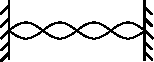
\includegraphics[width = 0.75in]{figures/stadbylgjanmin.pdf}
\end{wrapfigure}

\item \textit{(RK 17.5.)} Á myndinni hér til hægri má sjá staðbylgju sem sveiflast á streng af lengd $\ell = \SI{50}{cm}$ með tíðni $\SI{100}{Hz}$. Hver er bylgjuhraði bylgjunnar?

\end{minipage}


\begin{minipage}{\linewidth}

\begin{wrapfigure}{r}{1.8in}
\vspace{-0.5cm}
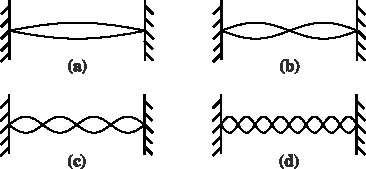
\includegraphics[width = 1.8in]{figures/standbert.pdf}
\end{wrapfigure}

\item \textit{(RK 17.6.)} Hér til hægri sjást fjórir mismunandi eiginsveifluhættir fyrir streng sem hefur lengd $\ell = \SI{2.0}{m}$ og línulegan þéttleika $\mu = \SI{1.5}{g/m}$. Strengurinn er festur á milli tveggja enda og togkrafturinn í strengnum er $T = \SI{2.4}{N}$. \begin{enumerate*}[label = \textbf{(\alph*)}]
    \item Hver er bylgjuhraðinn meðfram strengnum?
    \item Hverjar er bylgjulengdirnar fyrir hvern eiginsveifluhátt hér til hægri?
    \item Hverjar eru tilheyrandi eigintíðnir strengsins?
\end{enumerate*}

\end{minipage}

\begin{minipage}{\linewidth}

\begin{wrapfigure}{r}{1.3in}
\vspace{-1cm}
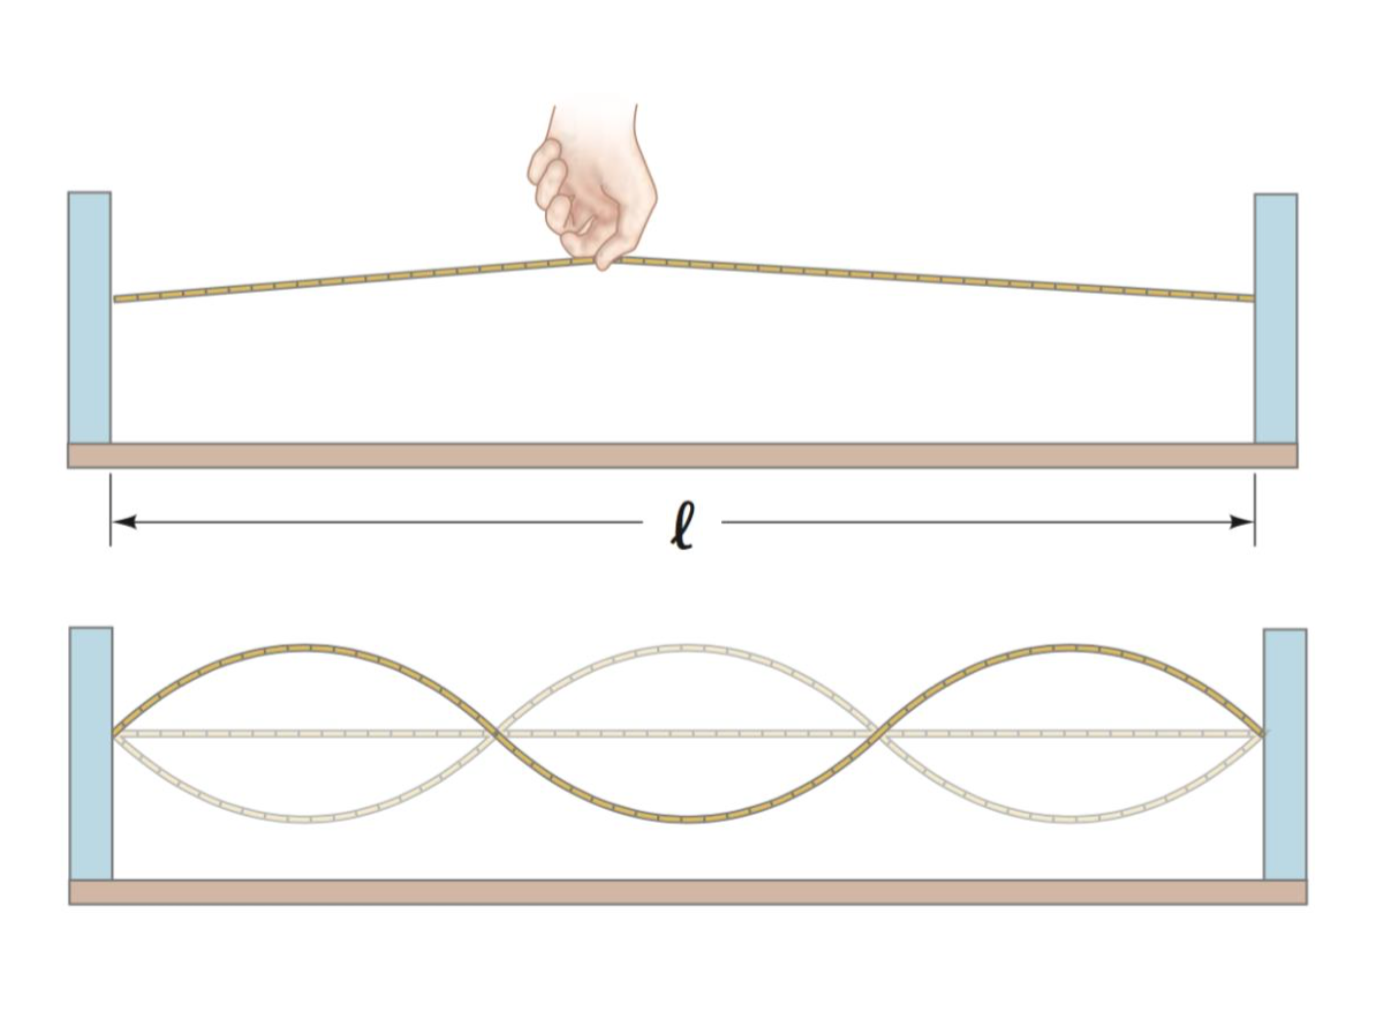
\includegraphics[width = 1.3in]{images/plokkun.png}
\end{wrapfigure}

\item Band með massa $m = \SI{1.6}{g}$ hangir milli tveggja stólpa sem eru í fjarlægð $\ell = \SI{0.60}{m}$ frá hvor öðrum. Finnið togkraftinn í bandinu þegar bandið sveiflast eins og á neðri myndinni hér til hægri með tíðni $\SI{1440}{Hz}$.

\item \textit{(RK 17.19.)} Líta má á klarínett sem sívalingslaga hálf-opið tréblásturshljóðfæri af lengd $\SI{100}{cm}$. Hver er grunntónn (fyrsta eigintíðni) klarínettsins? Hver er þriðji yfirtónn (þriðja eigintíðni) klarínettsins?

\end{minipage}

\begin{minipage}{\linewidth}

\begin{wrapfigure}{r}{1in}
\vspace{-0.5cm}
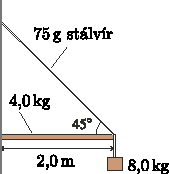
\includegraphics[width = 1in]{figures/copybest.pdf}
\end{wrapfigure}

\item \textit{(RK 17.48.)} Hver er grunntónn stálvírsins sem sést á uppstillingunni hér til hægri?

\item \textit{(RK 17.51.)} Við erum að skoða tvö mismunandi rör. Annað rörið er opið í báða enda og hefur lengd $\ell_1 = \SI{78.0}{cm}$. Hitt rörið er opið í annan endann og hefur lengd $\ell_2$. Í hálfopnu pípunni þá er fyrsti grunntónninn jafn þriðja yfirtón opnu pípunnar. Hver er lengd hálfopnu pípunnar?


\end{minipage}

\end{enumerate}

\subsection*{Svör}

\begin{enumerate*}[label = \vspace{0.15cm} \textbf{(\arabic*)}]
    \setcounter{enumi}{28}
  \item $\lambda = \SI{1.28}{m}$, $c = \SI{251}{m/s}$, $T = \SI{71.8}{N}$, $f = \SI{196}{Hz} $, $\lambda = \SI{1.75}{m}$.
  \item $c = \SI{25}{m/s}$.
  \item $c = \SI{40}{m/s}$, $\lambda_a = \SI{4.0}{m}$, $\lambda_b = \SI{2.0}{m}$, $\lambda_c = \SI{1.0}{m}$, $\lambda_d = \SI{50}{cm}$, $f_a = \SI{10}{Hz}$, $f_b = \SI{20}{Hz}$, $f_c = \SI{40}{Hz}$, $f_d = \SI{80}{Hz}$.
  \item $T = \SI{886}{N}$.
  \item $f_1 = \SI{86}{Hz}$, $f_3 = \SI{430}{Hz}$.
  \item $f_1 = \SI{12.8}{Hz}$.
  \item $\ell_2 = \SI{13.0}{cm}$.
\end{enumerate*}

\newpage


\subsection*{Bylgjusamliðun og hviður}

\begin{tcolorbox}
Við skoðuðum aðallega bylgjusamlagningu frá tveimur samfasa uppsprettum í fjarlægð $d$ frá hver annarri sem senda frá sér einsleitt hljóð með bylgjulengd $\lambda$ og tíðni $f$. Samliðunarbylgjan sem heyrist í punkti $P$ sem er í fjarlægð $r_1$ frá annarri uppsprettunni og $r_2$ frá hinni er þá:
\begin{align*}
    A\sin(kr_1-\omega t) + A\sin(kr_2 - \omega t) = 2A\cos(\frac{1}{2}k\Delta r)\sin(\frac{1}{2}k(r_1+r_2)-\omega t)
\end{align*}
Sér í lagi sáum við að fyrir fullkomlega styrkjandi/eyðjandi samliðun þá gildir að:
\begin{align*}
    \Delta r = \begin{cases}
    n \lambda \hspace{2.8cm} \text{(styrkjandi bylgjusamliðun)} \\
    \left(n+\frac{1}{2}\right)\lambda \hspace{1.8cm} \text{(eyðandi bylgjusamliðun)}
    \end{cases},\hspace{1cm} n \in \N.
\end{align*}
Hviðutíðnin $\Delta f = f_2 - f_1$ heyrist þegar tveir tónar, $f_1$ og $f_2$ eru örlítið frábrugðnir ($f_1 \approx f_2$).
\end{tcolorbox}

\begin{enumerate}[label = \textbf{Dæmi \thechapter.\arabic*.}]
\setcounter{enumi}{35}

\begin{comment}
\item \textit{(RK. 17.24.)} Active Noise Cancelling (ANC) heyrnartól eru vinsæll ferðafélagi í flugferðum. Það er útaf hljóðeinangruninni sem útilokar öll umhverfishljóð fyrir þann sem notar þau. En hvernig virka slík heyrnartól? Þau byggja á því að á hvorri hlið heyrnartólanna er lítill hljóðnemi sem greinir utanaðkomandi hljóð og bætir síðan við umsnúnu hljóðbylgjunni (samlagningarandhverfa hljóðbylgjunnar frá umhverfinu) í hljóðið sem við heyrum (og þar með heyrum ekki!). Einfaldasta leiðin til þess að bæta við umsnúnu hljóðbylgjunni er bara að senda út sama hljóðmerki með örlítilli seinkunn þannig að fasamunurinn á milli hljóðbylgnanna gefur eyðandi bylgjusamliðun. Hversu mikil á þessi tímaseinkun, $\tau$, að vera ef flugvélarhreyflarnir senda frá sér pirrandi hljóð með tíðni $f = \SI{380}{Hz}$?
\end{comment}

\item \textit{(RK 17.29.)} Tveir hátlarar sem eru í fasa við hvorn annan senda frá sér einsleittan tón með tíðni $f$ í allar stefnur. Nú færum við annan þeirra $\SI{3.0}{m}$ til hægri og $\SI{4.0}{m}$ áfram miðað við hinn hátlarann. Eftir að við erum búin að færa hátlarana þá heyrist (ekki) eyðandi bylgjusamliðun í $\frac{1}{4}$ og $\frac{3}{4}$ af vegalengdinni á milli hátlaranna á stystu línunni milli þeirra. Hver er lengsta mögulega bylgjulengd sem að hljóðbylgjurnar hafa og hver er tíðni hljóðsins?

\begin{minipage}{\linewidth}

\begin{wrapfigure}{r}{1.3in}
\vspace{-0.75cm}
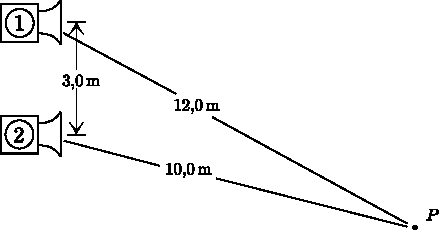
\includegraphics[width = 1.3in]{figures/dia-hatalar.pdf}
\end{wrapfigure}

\item Tveir hátlarar sem eru í fjarlægð $\SI{3.0}{m}$ frá hvorum öðrum spila einsleitt, samfasa hljóð með tíðni $f$. Þú stendur í punkti $P$ sem er í fjarlægð $r_1 = \SI{12.0}{m}$ frá öðrum hátalaranum og fjarlægð $r_2 = \SI{10.0}{m}$ frá hinum hátalaranum og heyrir ekkert hljóð! Hver er lægsta mögulega tíðni sem hátalararnir geta haft?

\end{minipage}

\begin{minipage}{\linewidth}

\begin{wrapfigure}{r}{1in}
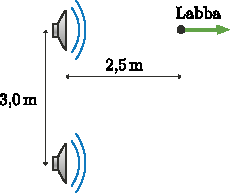
\includegraphics[width = 1in]{figures/micron.pdf}
\end{wrapfigure}

\item Tveir hátalarar senda frá sér einsleitt, samfasa hljóð með tíðni $f = \SI{500}{Hz}$ og útslag $A = \SI{0.10}{mm}$. Hátlararnir eru í $\SI{1.0}{m}$ fjarlægð frá hvor öðrum og þú stendur í $\SI{1.0}{m}$ fjarlægð frá öðrum þeirra og $\SI{2.0}{m}$ fjarlægð frá hinum (í beinni línu). Hvert er útslag samliðunarbylgjunnar sem þú heyrir frá hátölurunum? Er þetta styrkjandi eða eyðandi bylgjusamliðun?

\item \textit{(RK 17.68.)} Tveir hátlarar sem eru í fjarlægð $\SI{3.0}{m}$ frá hvorum öðrum spila samfasa hljóð með tíðni $f = \SI{686}{Hz}$. Þú stendur $\SI{2.5}{m}$ beint fyrir framan annan hátalarann og byrjar að labba beint í burtu. Hversu langt þarftu að labba til þess að heyra eyðandi bylgjusamliðun?


\end{minipage}



\item \textit{(RK 17.32.)} Tveir strengir eru stilltir þannig að þeir gefi frá sér hljóð með tíðni $\SI{200}{Hz}$. Nú herðum við togkraftinn í öðrum strengnum þannig að það heyrast þrjár hviður á hverri sekúndu þegar að við sláum á strengina. Hver er tíðni strengsins þar sem togkrafturinn var hertur?

\begin{minipage}{\linewidth}

\begin{wrapfigure}{r}{1.7in}
\vspace{-0.75cm}
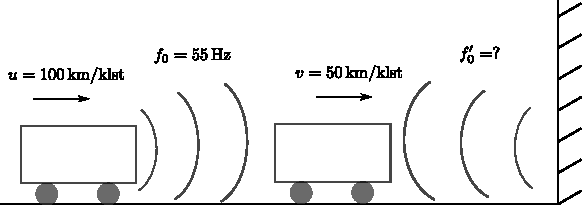
\includegraphics[width = 1.7in]{figures/eftirfor-irodov.pdf}
\end{wrapfigure}

\item Lögregluþjónn er að veita mannræningjum eftirför. Hann keyrir í áttina að mannræningjunum með hraða $u = \SI{100}{km/klst}$ með kveikt á sírenu sem sendir út hljóð með tíðni $f_0 = \SI{55}{Hz}$. Mannræningjarnir keyra með hraða $v = \SI{50}{km/klst}$. Lögregluþjónninn er búinn að króa mannræningjana af þannig að nú stefna þeir beint í áttina að risastóru bjargi. Hljóðbylgjurnar endurvarpast af bjarginu. \begin{enumerate*}[label = \textbf{(\alph*)}]
    \item Hvaða tíðni, $f_1$, heyra mannræningjarnir frá sírenum lögregluþjónsins?
    \item Hver er tíðni endurvörpuðu bylgjunnar, $f_0'$ frá veggnum?
    \item Hvaða tíðni, $f_2$, heyra mannræningjarnir frá endurvörpuðu hljóðbylgjunni?
    \item Hver er hviðutíðnin $\Delta f = f_2 - f_1$ sem mannræningjarnir heyra?
\end{enumerate*}  

\end{minipage}

\end{enumerate}

\subsection*{Svör}

\begin{enumerate*}[label = \vspace{0.15cm} \textbf{(\arabic*)}]
    \setcounter{enumi}{35}
  \item $\lambda = \SI{5.0}{m}$, $f = \SI{69}{Hz}$.
  \item $f_{\text{min}} = \SI{86}{Hz}$.
  \item $B = \SI{26}{\mu m}$.
  \item $\Delta x = \SI{48}{cm}$.
  \item $f = \SI{203}{Hz}$
  \item $f_1 = \SI{57}{Hz}$, $f_0' = \SI{60}{Hz}$, $f_2 = \SI{62}{Hz}$, $\Delta f = \SI{4.8}{Hz}$.
\end{enumerate*}


%%%%%%%%%%%%%%%%%%%%%%%%%%%%%%%%
%      END OF CHAPTER TEXT 
%%%%%%%%%%%%%%%%%%%%%%%%%%%%%%%%
\ifdefined \wholebook \else
 \printindex
\end{document}
\fi